\begin{figure}
\begin{adjustwidth}{-0.8in}{-0.5in}  
    \centering                     
    \footnotesize
\setlength\tabcolsep{2pt}
\vspace{-0.5in}
\begin{tabular}{cccccccccccccccccccc}

\multicolumn{3}{c}{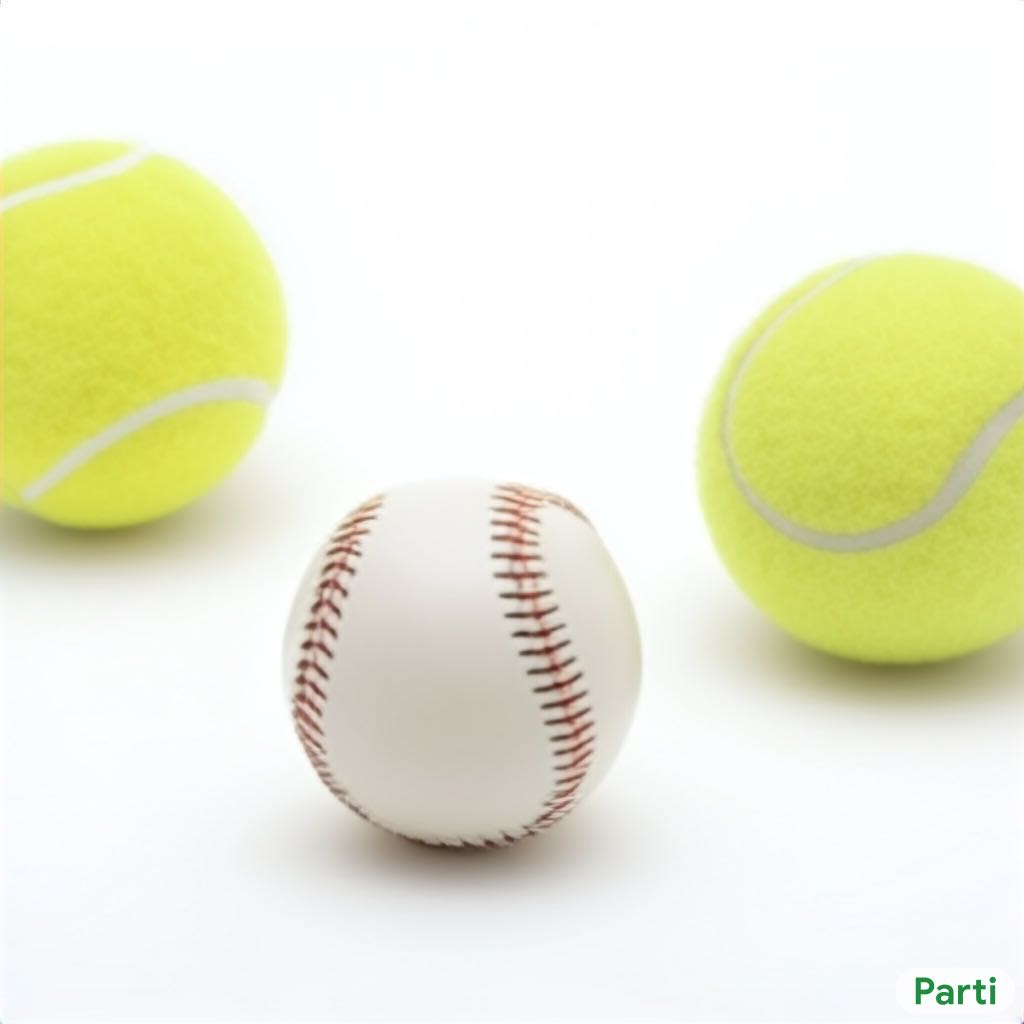
\includegraphics[width=\twobytwocolwidth\textwidth]{figures/limitations/2tennis1baseball.jpg}} &
\multicolumn{3}{c}{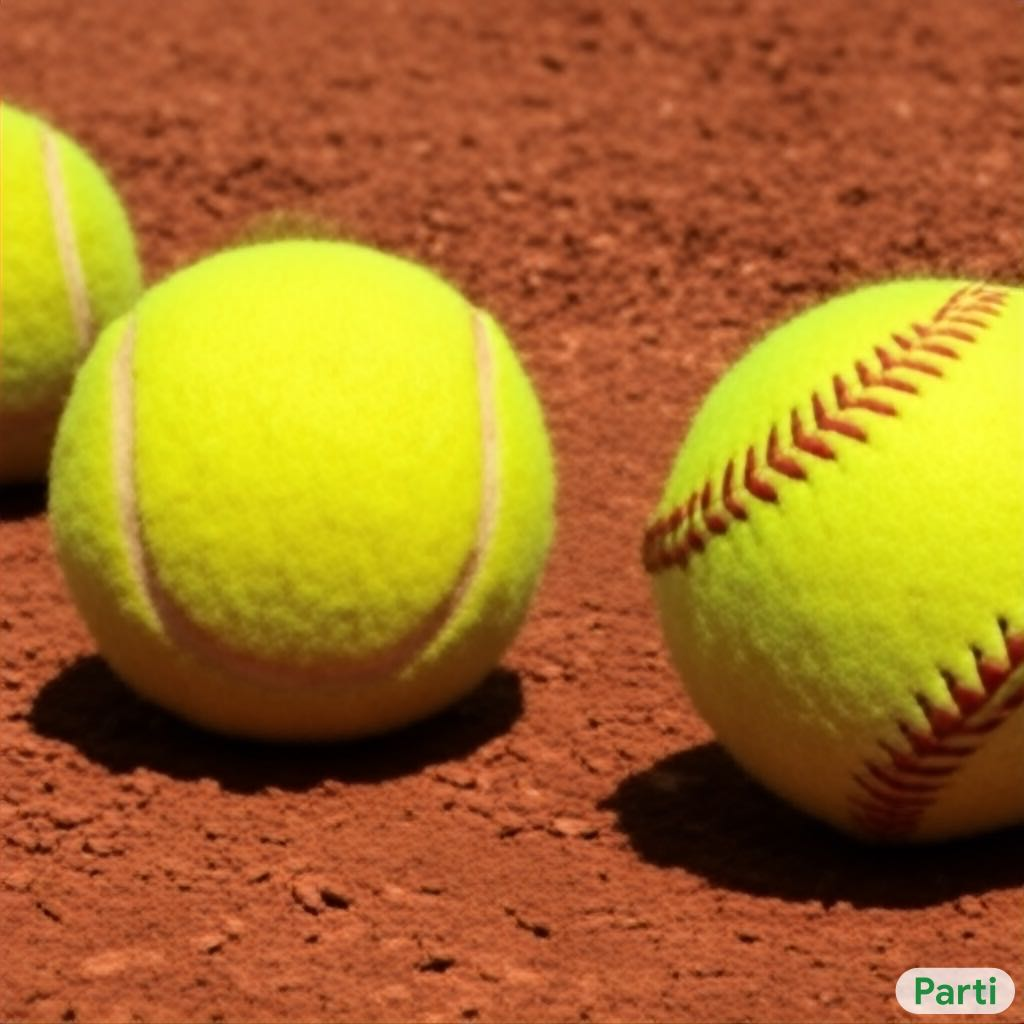
\includegraphics[width=\twobytwocolwidth\textwidth]{figures/limitations/2tennis1mergedball.jpg}} &&
\multicolumn{3}{c}{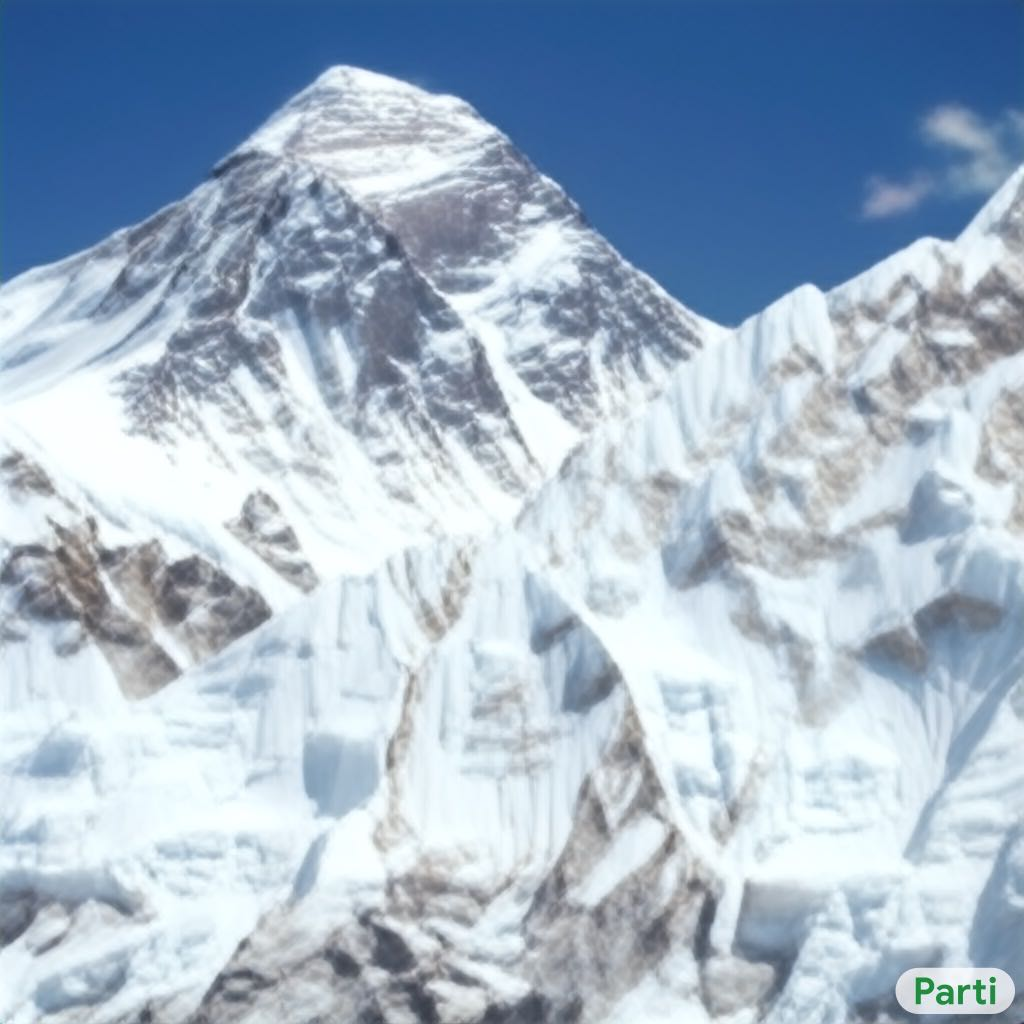
\includegraphics[width=\twobytwocolwidth\textwidth]{figures/limitations/everest_only.jpg}} &
\multicolumn{3}{c}{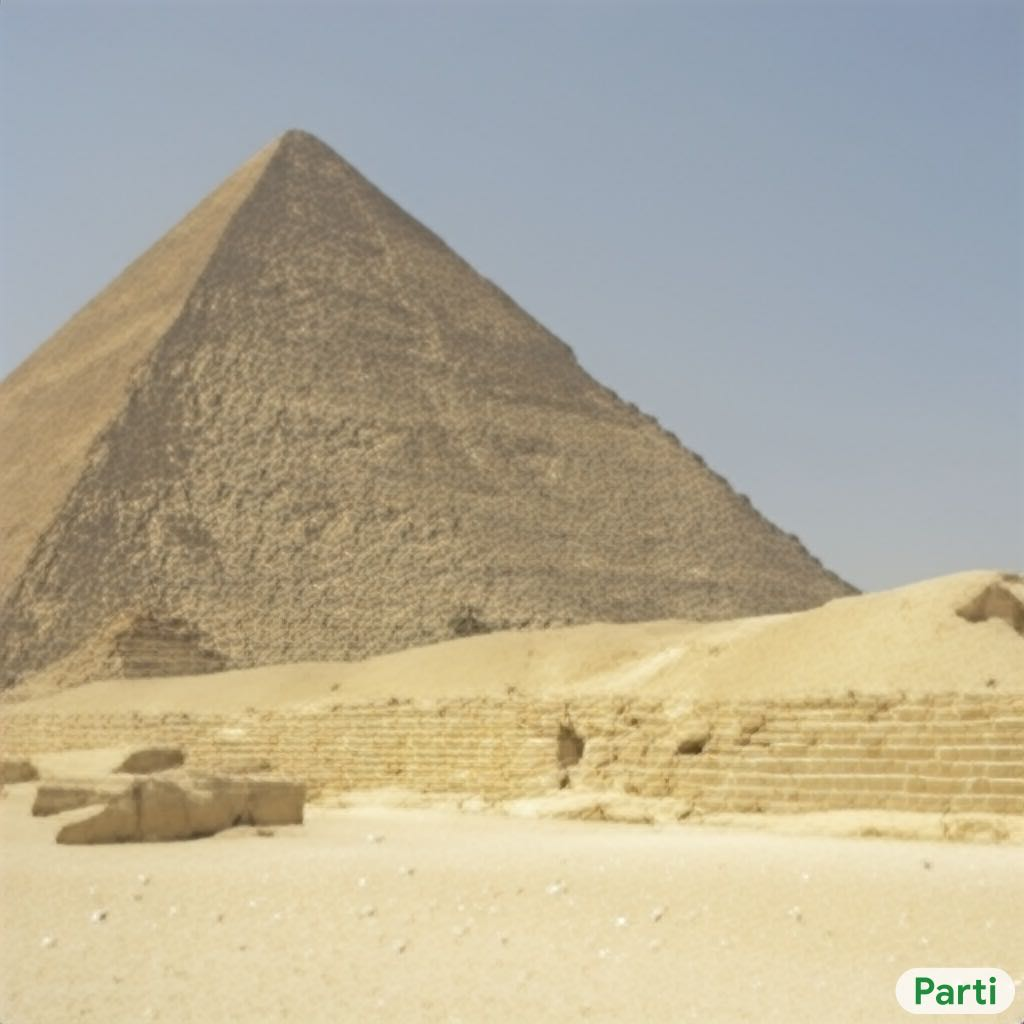
\includegraphics[width=\twobytwocolwidth\textwidth]{figures/limitations/pyramid_only.jpg}} &&
\multicolumn{3}{c}{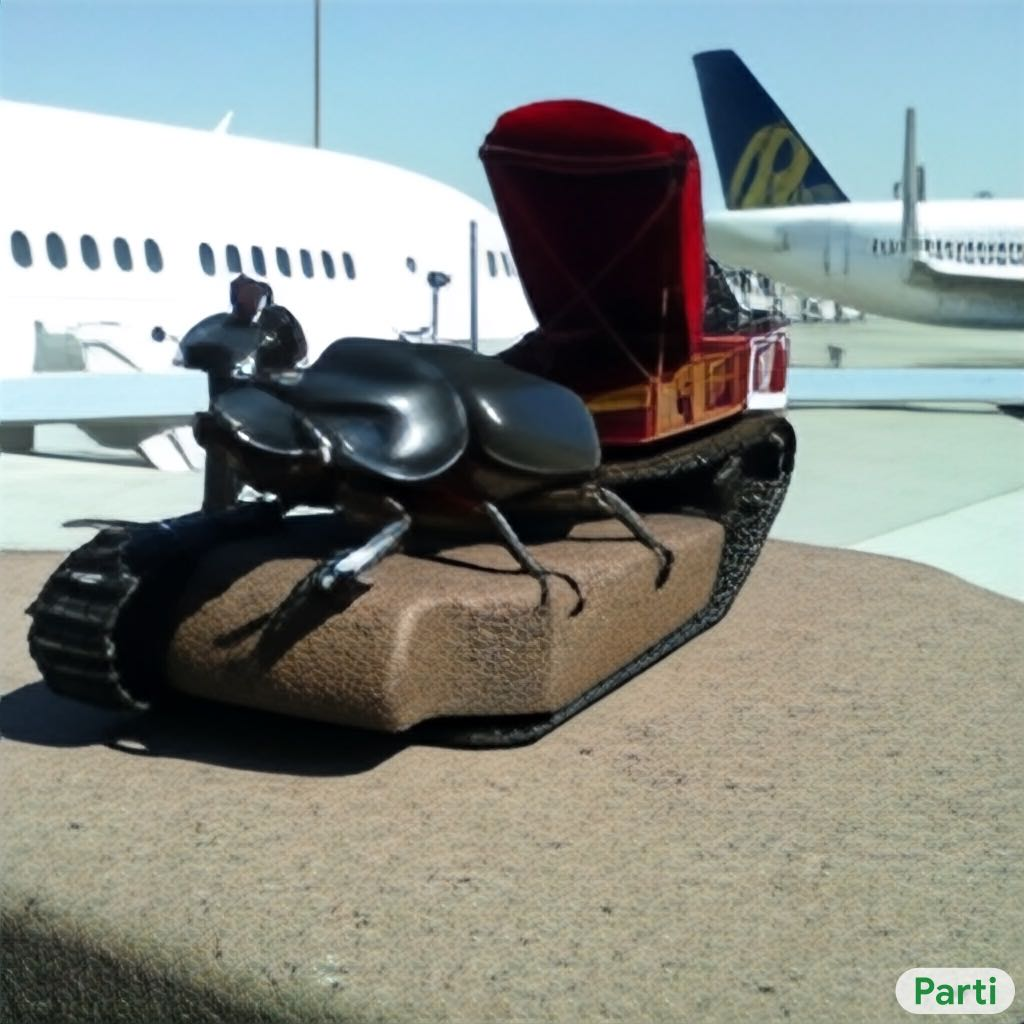
\includegraphics[width=\twobytwocolwidth\textwidth]{figures/limitations/rhino1.jpg}} &
\multicolumn{3}{c}{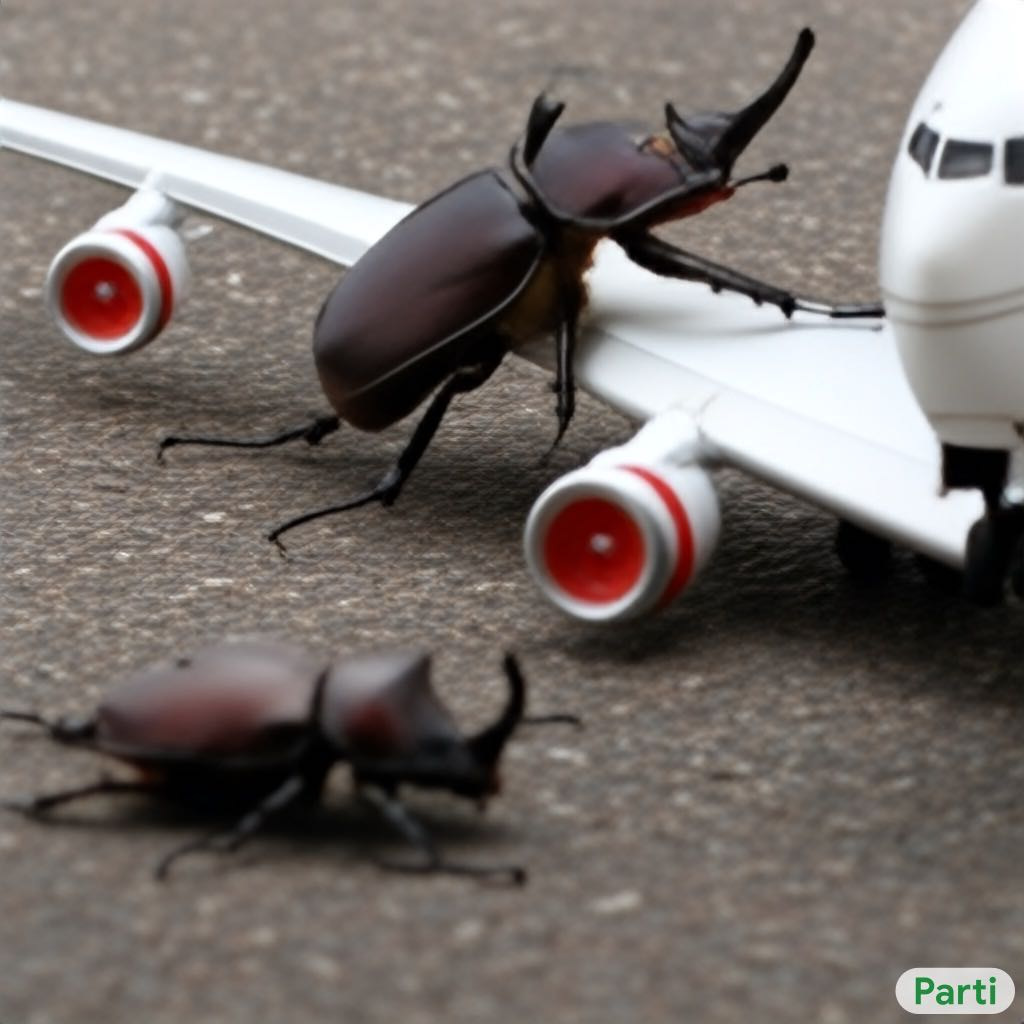
\includegraphics[width=\twobytwocolwidth\textwidth]{figures/limitations/rhino2.jpg}} \\
\multicolumn{3}{c}{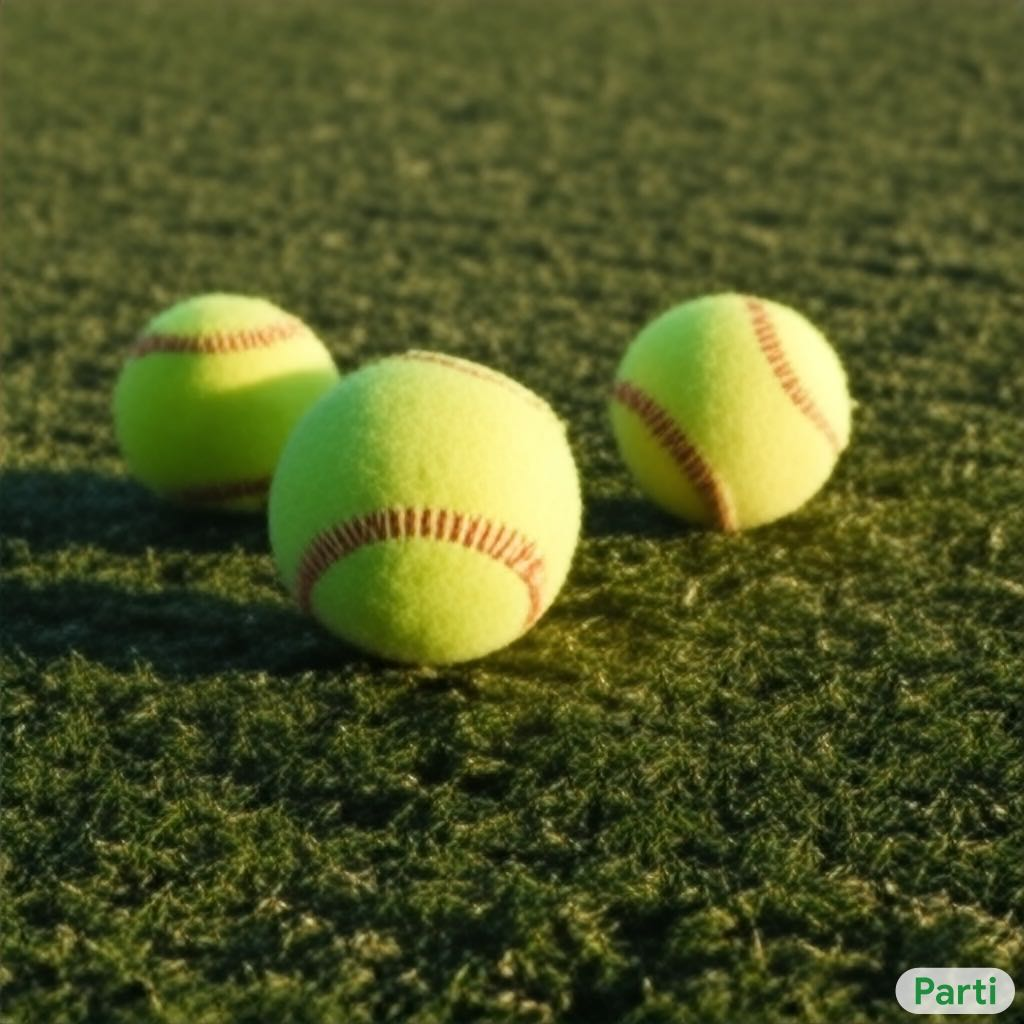
\includegraphics[width=\twobytwocolwidth\textwidth]{figures/limitations/3mergedballs.jpg}} &
\multicolumn{3}{c}{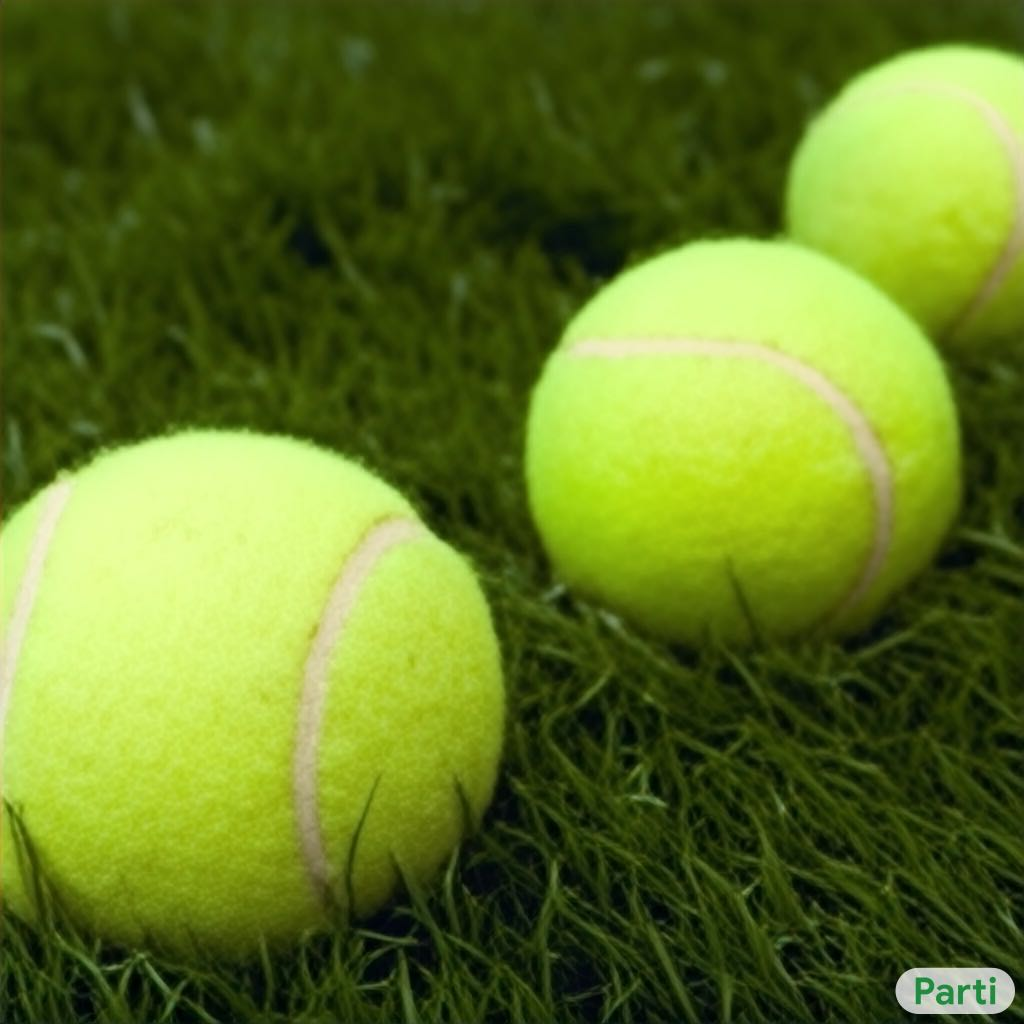
\includegraphics[width=\twobytwocolwidth\textwidth]{figures/limitations/3tennisballs.jpg}} &&
\multicolumn{3}{c}{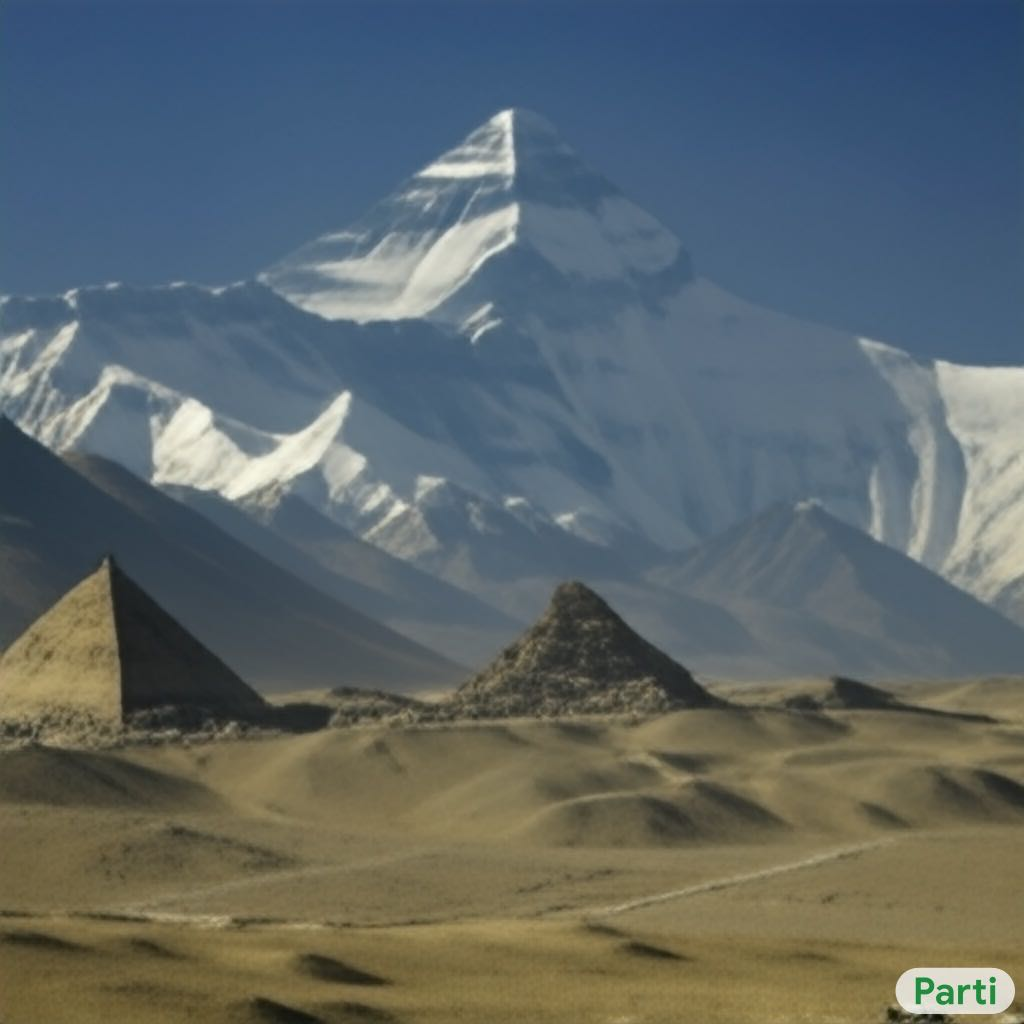
\includegraphics[width=\twobytwocolwidth\textwidth]{figures/limitations/everent_pyramid_merge1.jpg}} &
\multicolumn{3}{c}{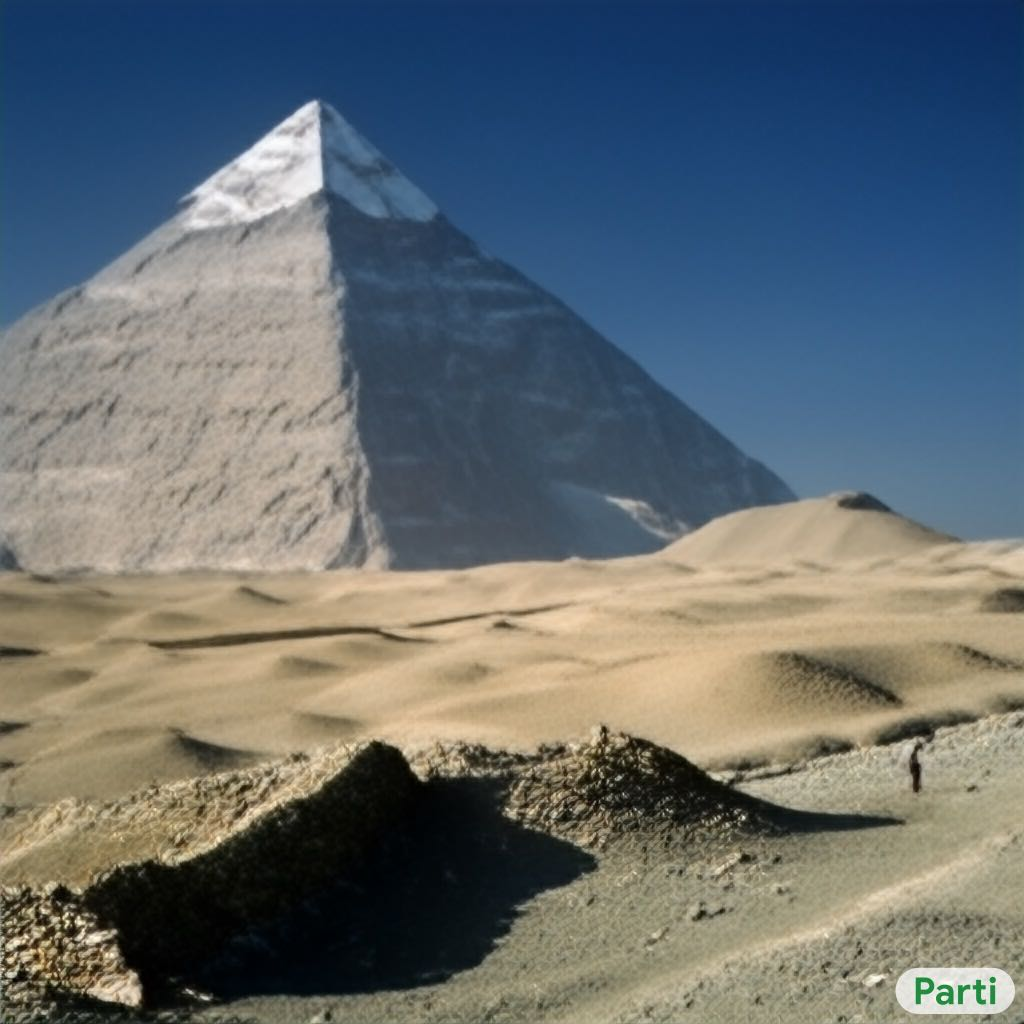
\includegraphics[width=\twobytwocolwidth\textwidth]{figures/limitations/everest_pyramid_merge2.jpg}} &&
\multicolumn{3}{c}{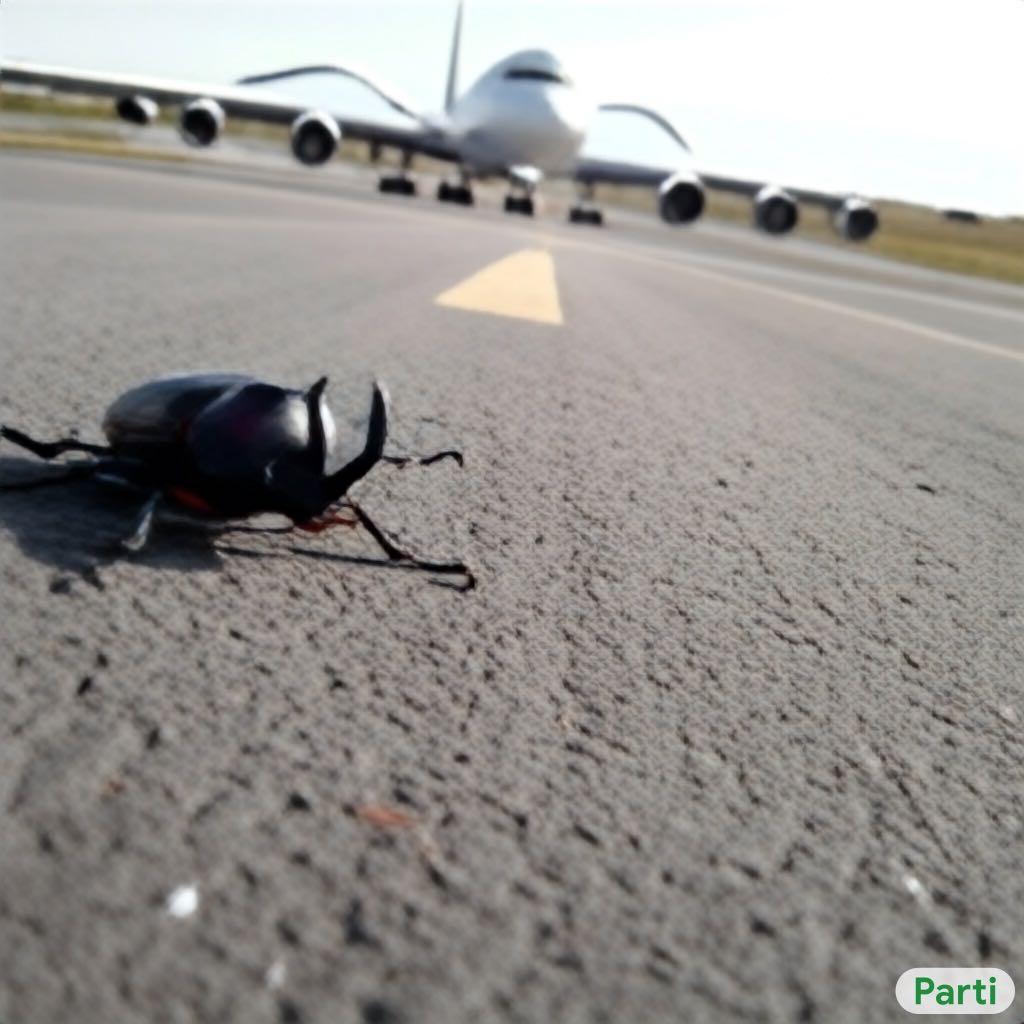
\includegraphics[width=\twobytwocolwidth\textwidth]{figures/limitations/rhino3.jpg}} &
\multicolumn{3}{c}{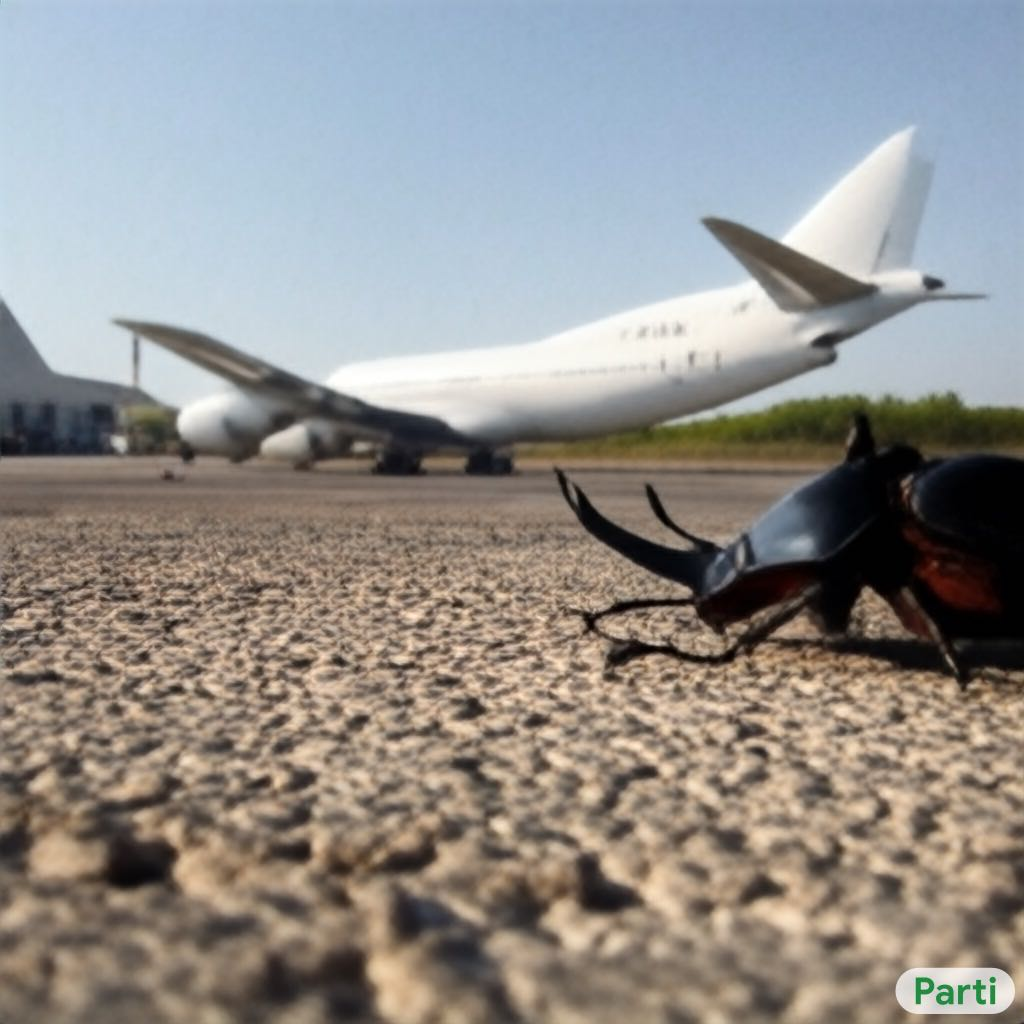
\includegraphics[width=\twobytwocolwidth\textwidth]{figures/limitations/rhino4.jpg}} \\
\multicolumn{6}{C{\thirdcolwidth\textwidth}}{\tiny \textbf{A}. Four images generated in the same batch for the prompt  \textit{two baseballs to the left of three tennis balls}. \textbf{Failures}: color bleeding (b); feature merging (b,c); counting (a-d); spatial relations (a-d). (b-d) also include (arguably reasonable) hallucination of ground details such as gravel and grass.} && 
\multicolumn{6}{C{\thirdcolwidth\textwidth}}{\tiny \textbf{B}. Generated images of (a) \textit{Mount Everest} and (b) \textit{The Great Pyramid} as references and demonstrating the model's knowledge. Two images (c,d) generated for \textit{The Great Pyramid of Giza situated in front of Mount Everest.} \textbf{Failures}: feature-merging of pyramid with pyramidal top of Everest (d) or making a snowy Egyptian Pyramid (d); the pyramid depicted is Khafre's, not Khufu's (Great) Pyramid (d).} && 
\multicolumn{6}{C{\thirdcolwidth\textwidth}}{\tiny \textbf{C}. Four images generated in the same batch for the prompt  \textit{A rhino beetle this size of a tank grapples a real life passenger airplane on the tarmac.} \textbf{Failures}: difficulty in overriding true life size leads to a big beetle poorly merged with a tank (a); toy airplane (b), attempts to use perspective to make a big beetle (c,d), hallucination of extra beetle (b).} \\

\multicolumn{3}{c}{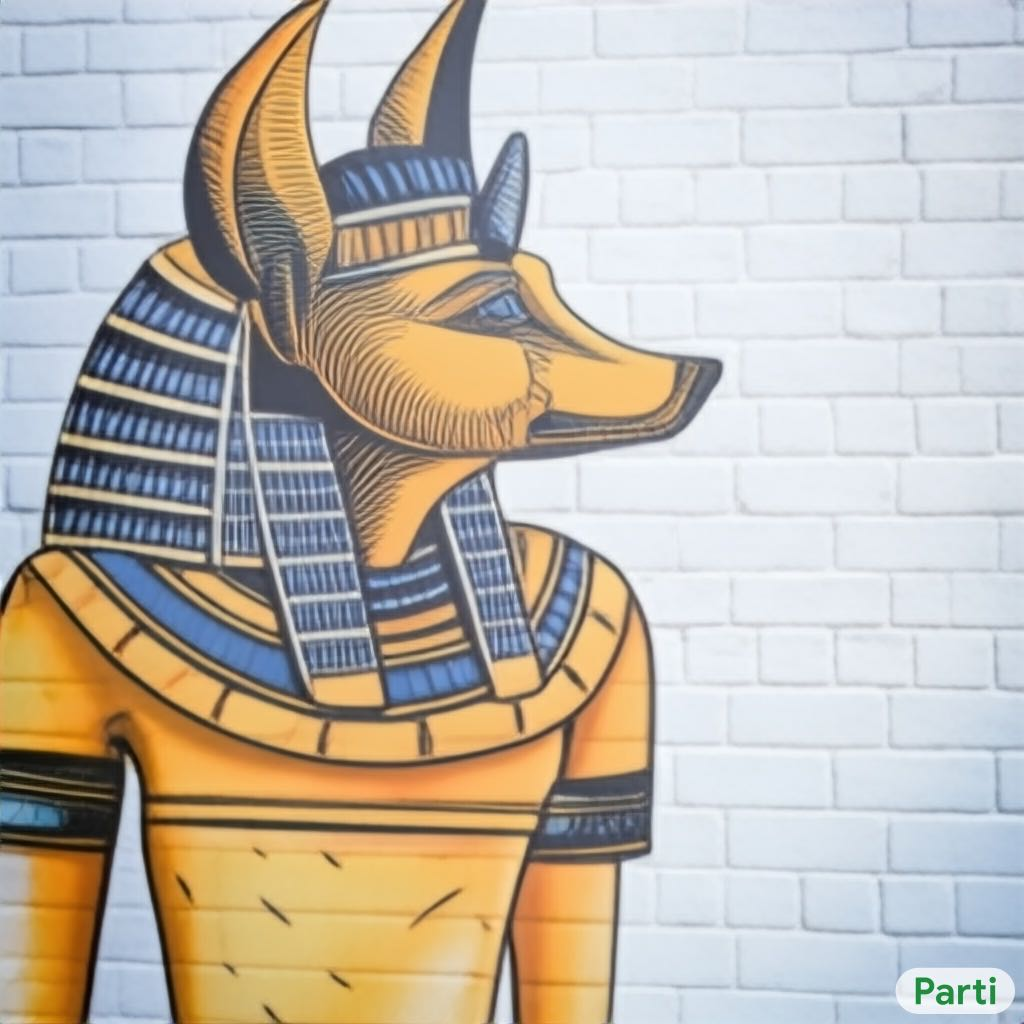
\includegraphics[width=\twobytwocolwidth\textwidth]{figures/limitations/yellow_anubis1.jpg}} &
\multicolumn{3}{c}{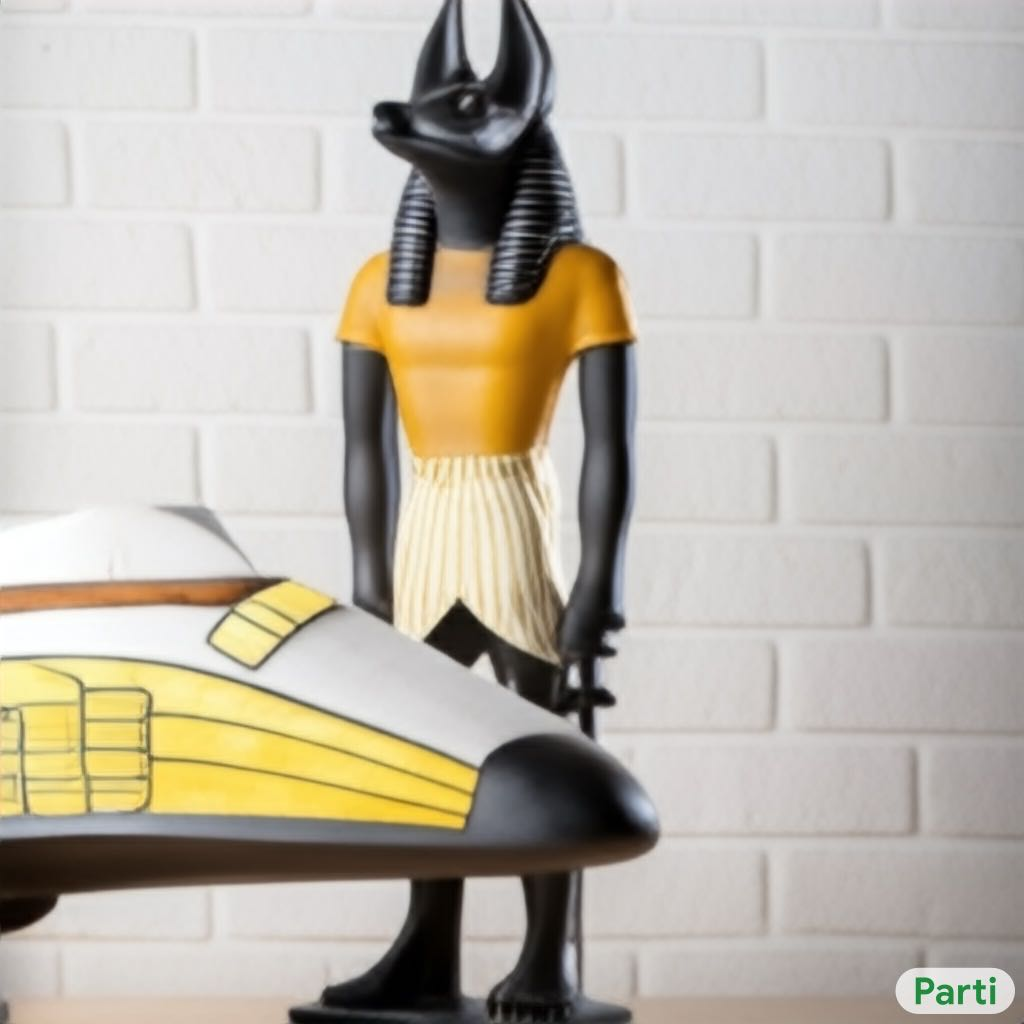
\includegraphics[width=\twobytwocolwidth\textwidth]{figures/limitations/yellow_anubis2.jpg}} &&
\multicolumn{3}{c}{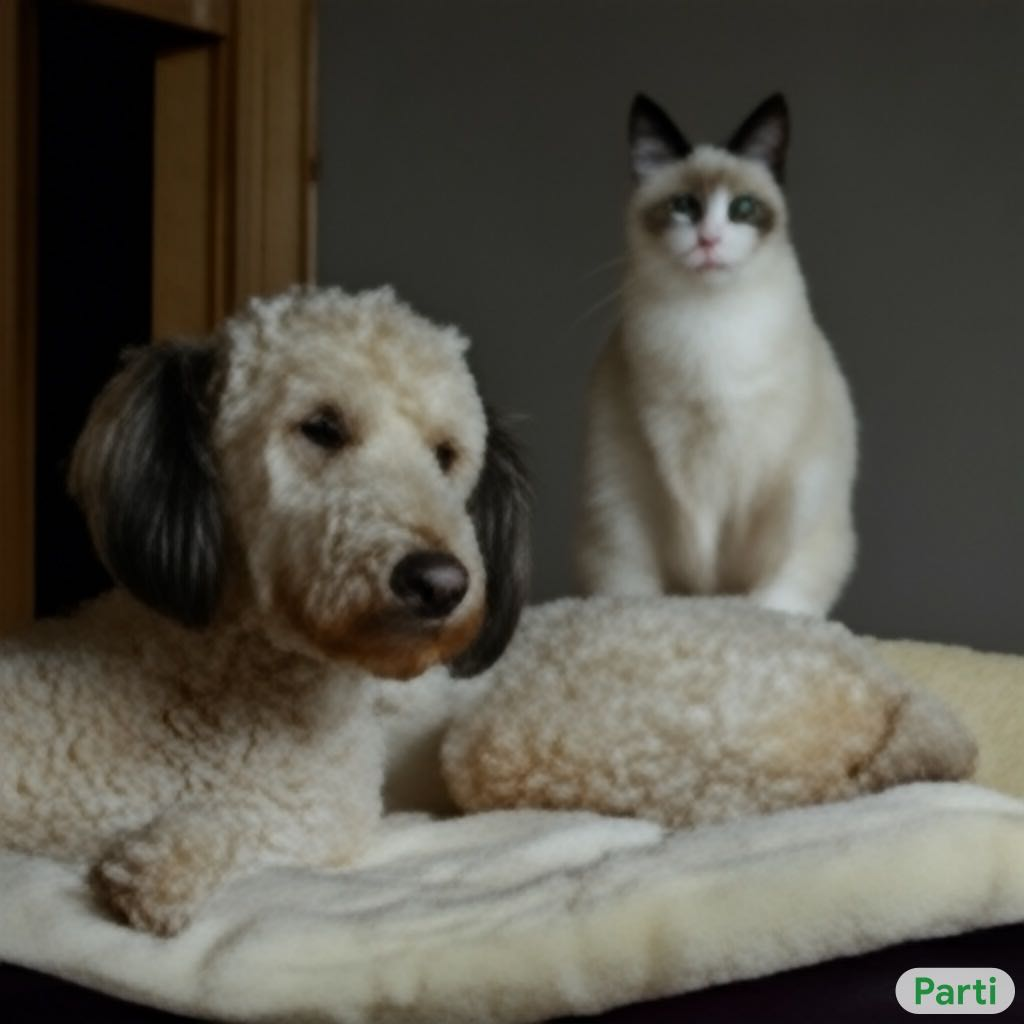
\includegraphics[width=\twobytwocolwidth\textwidth]{figures/limitations/labra_cat1.jpg}} &
\multicolumn{3}{c}{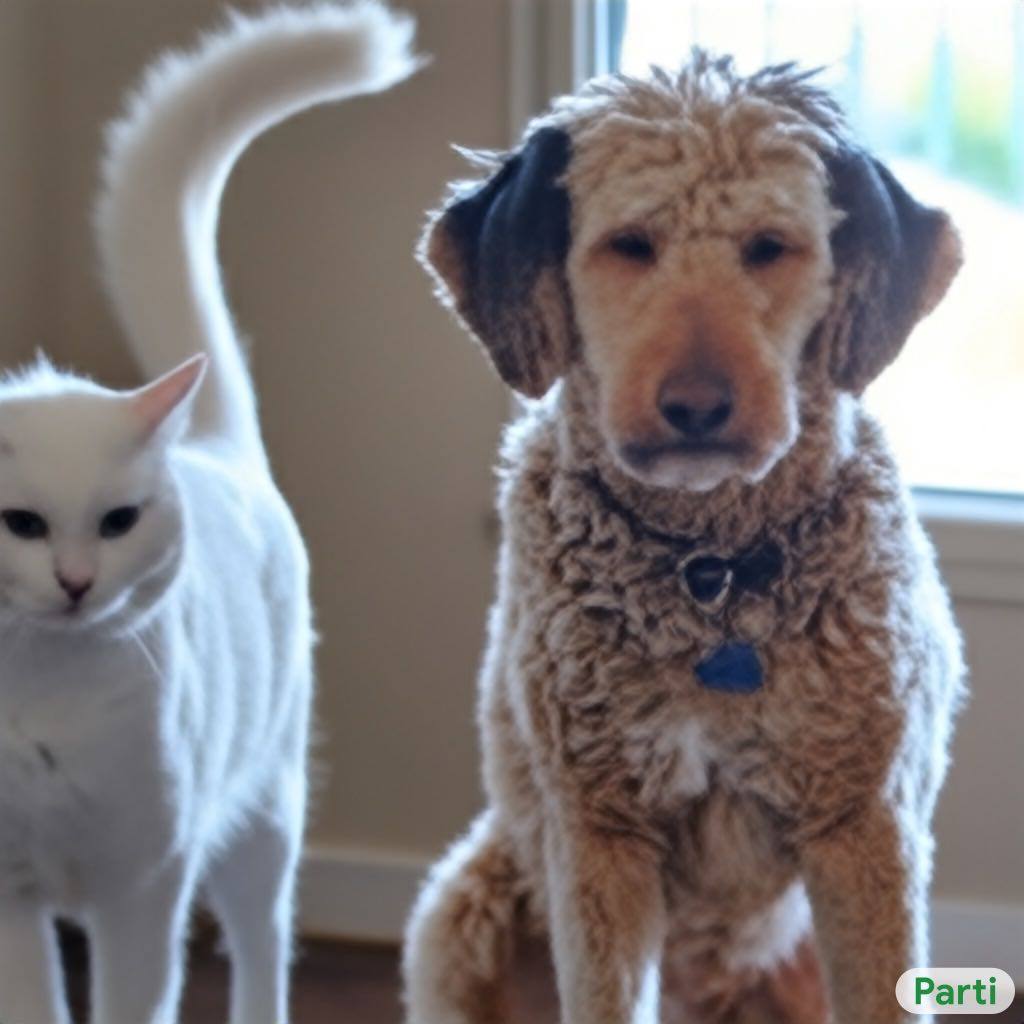
\includegraphics[width=\twobytwocolwidth\textwidth]{figures/limitations/labra_cat4.jpg}} &&
\multicolumn{3}{c}{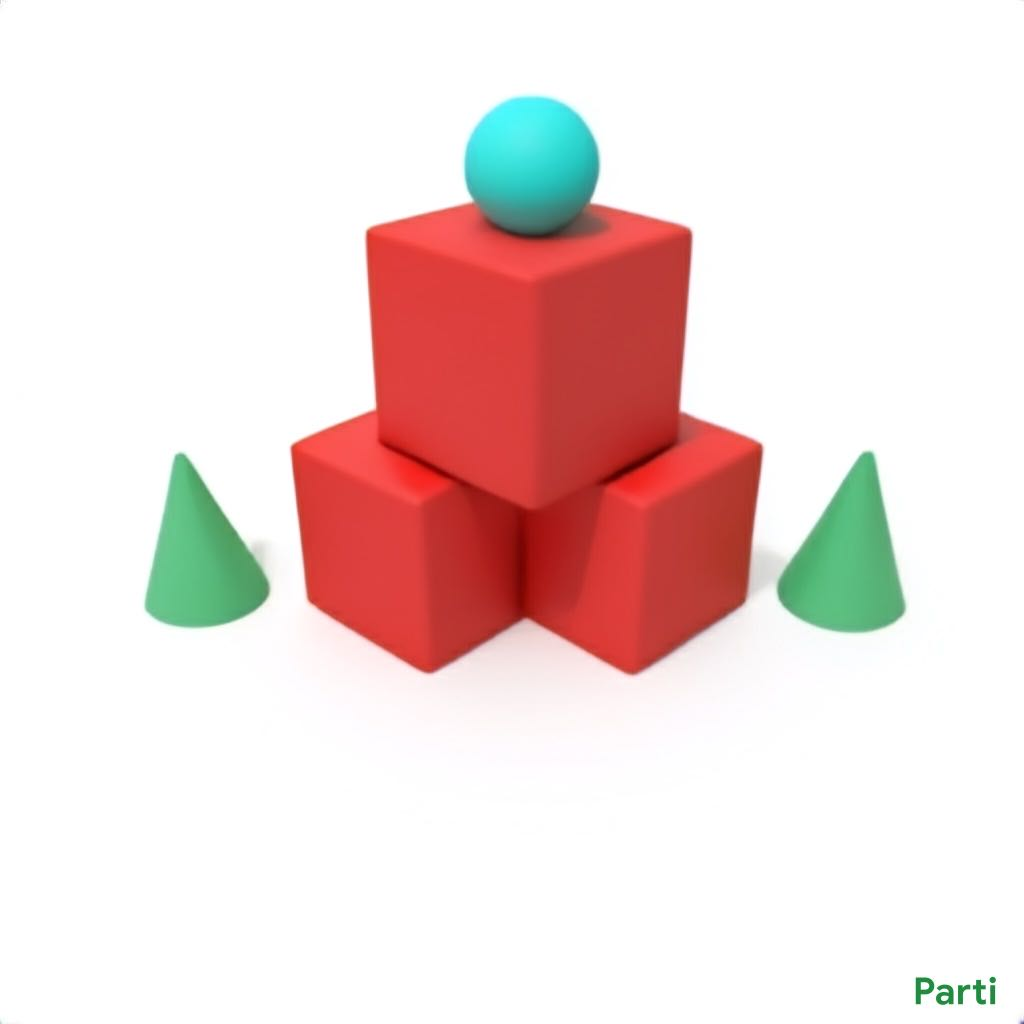
\includegraphics[width=\twobytwocolwidth\textwidth]{figures/limitations/cube_cone1.jpg}} &
\multicolumn{3}{c}{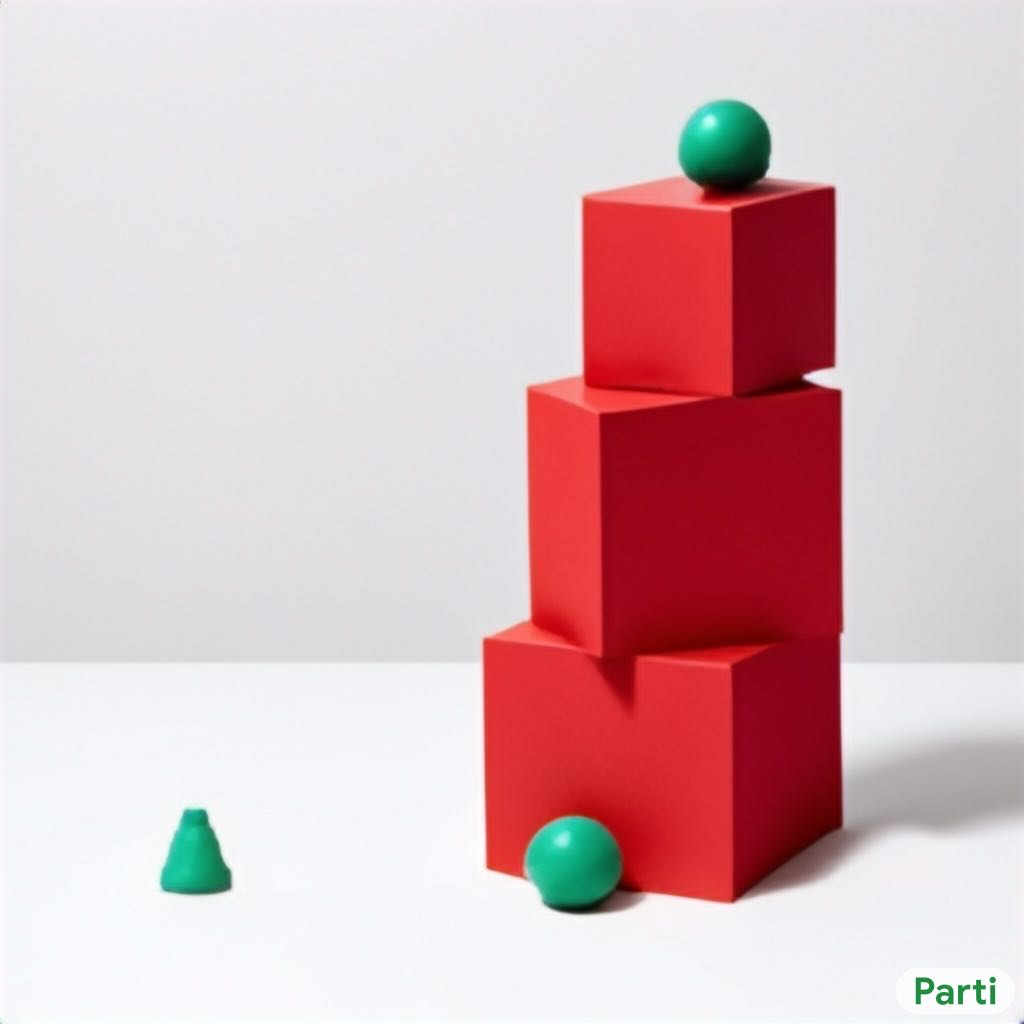
\includegraphics[width=\twobytwocolwidth\textwidth]{figures/limitations/cube_cone2.jpg}} \\
\multicolumn{3}{c}{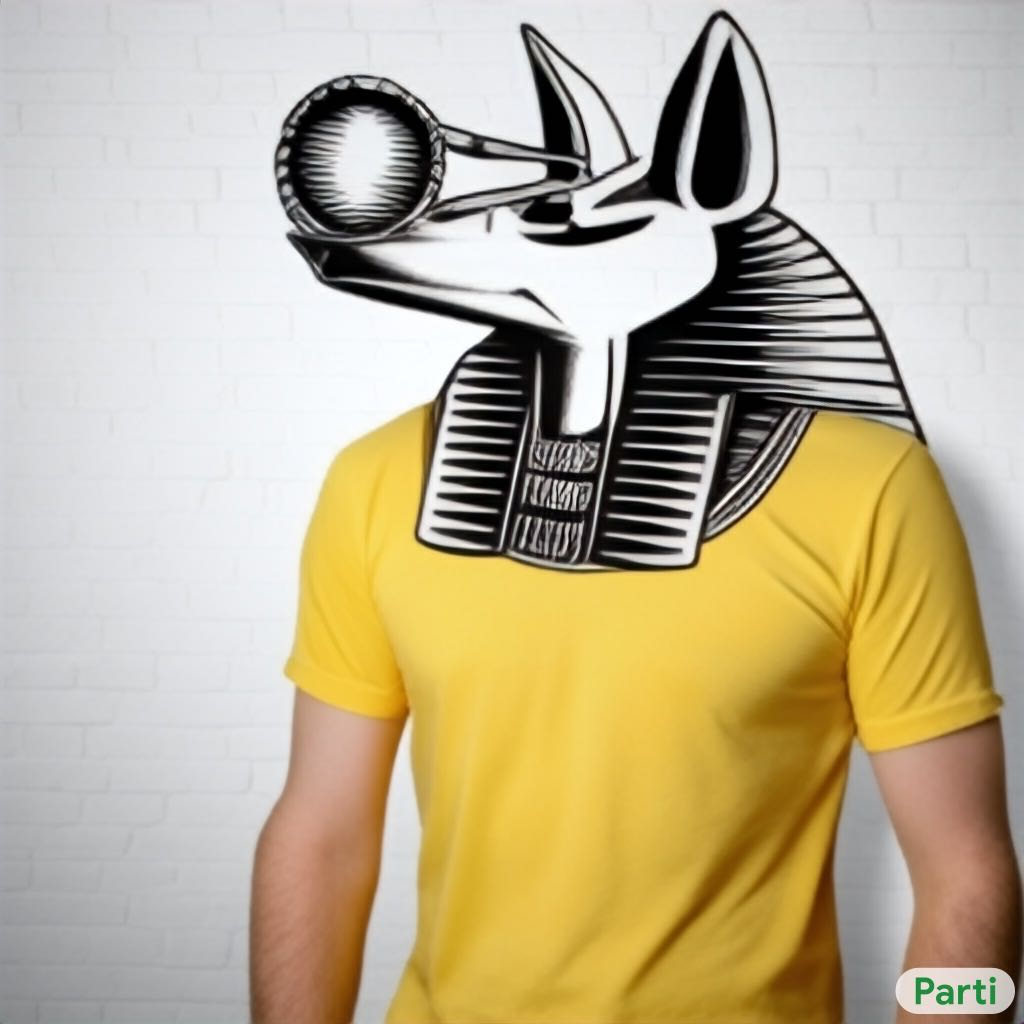
\includegraphics[width=\twobytwocolwidth\textwidth]{figures/limitations/yellow_anubis3.jpg}} &
\multicolumn{3}{c}{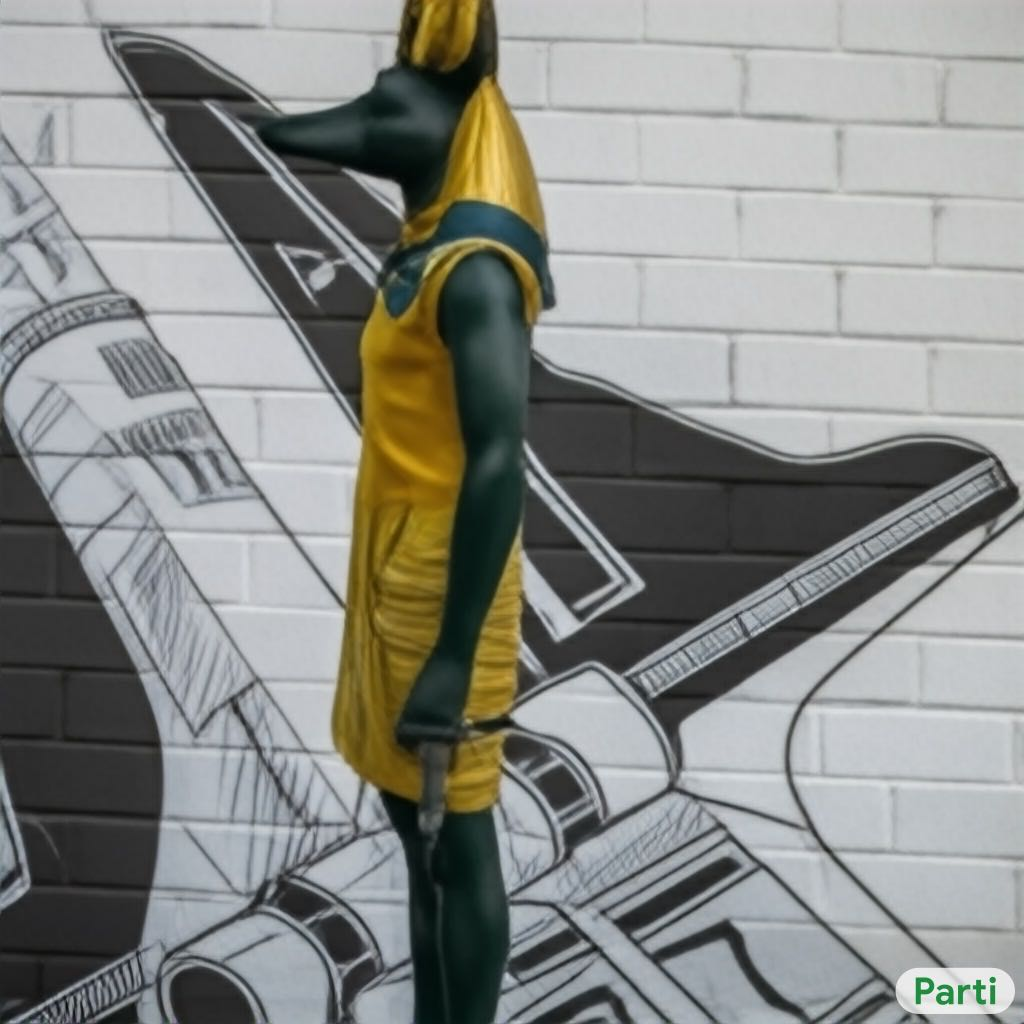
\includegraphics[width=\twobytwocolwidth\textwidth]{figures/limitations/yellow_anubis4.jpg}} &&
\multicolumn{3}{c}{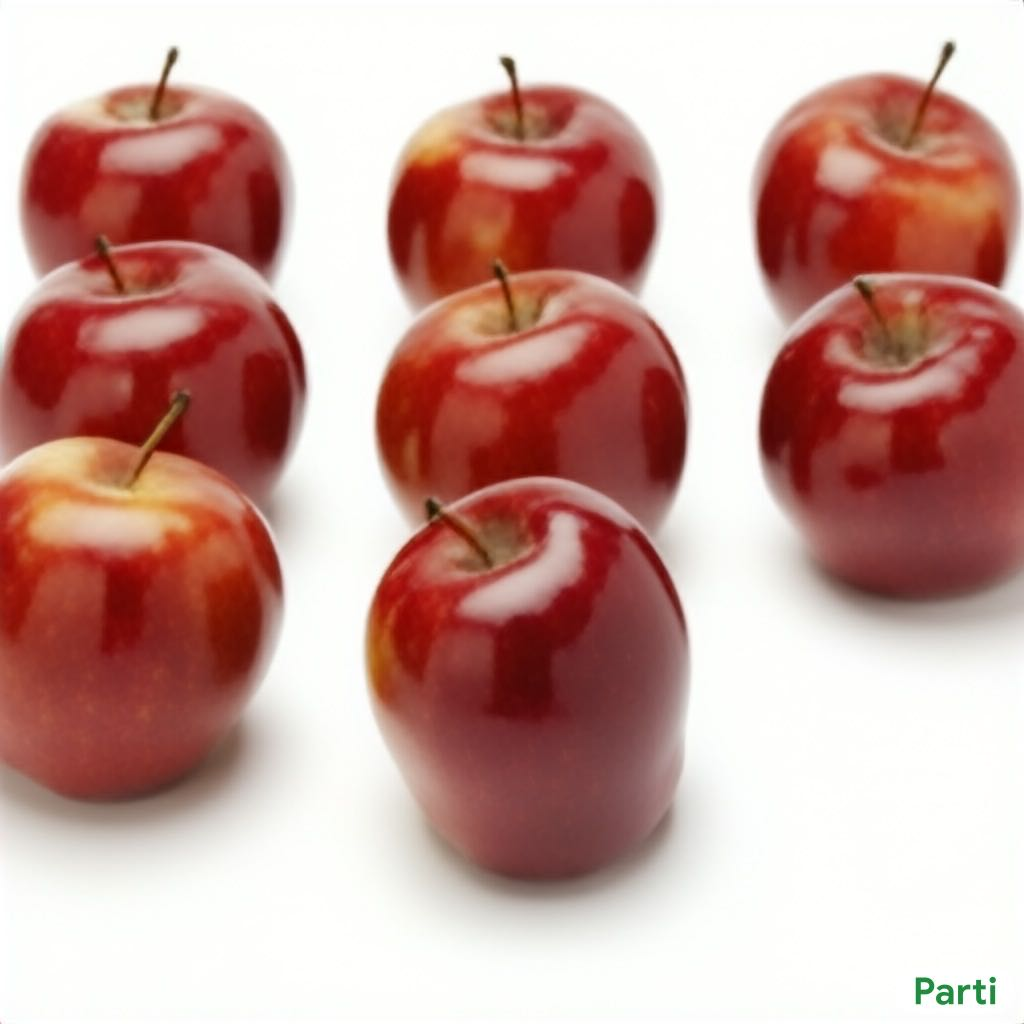
\includegraphics[width=\twobytwocolwidth\textwidth]{figures/limitations/apples_count8.jpg}} &
\multicolumn{3}{c}{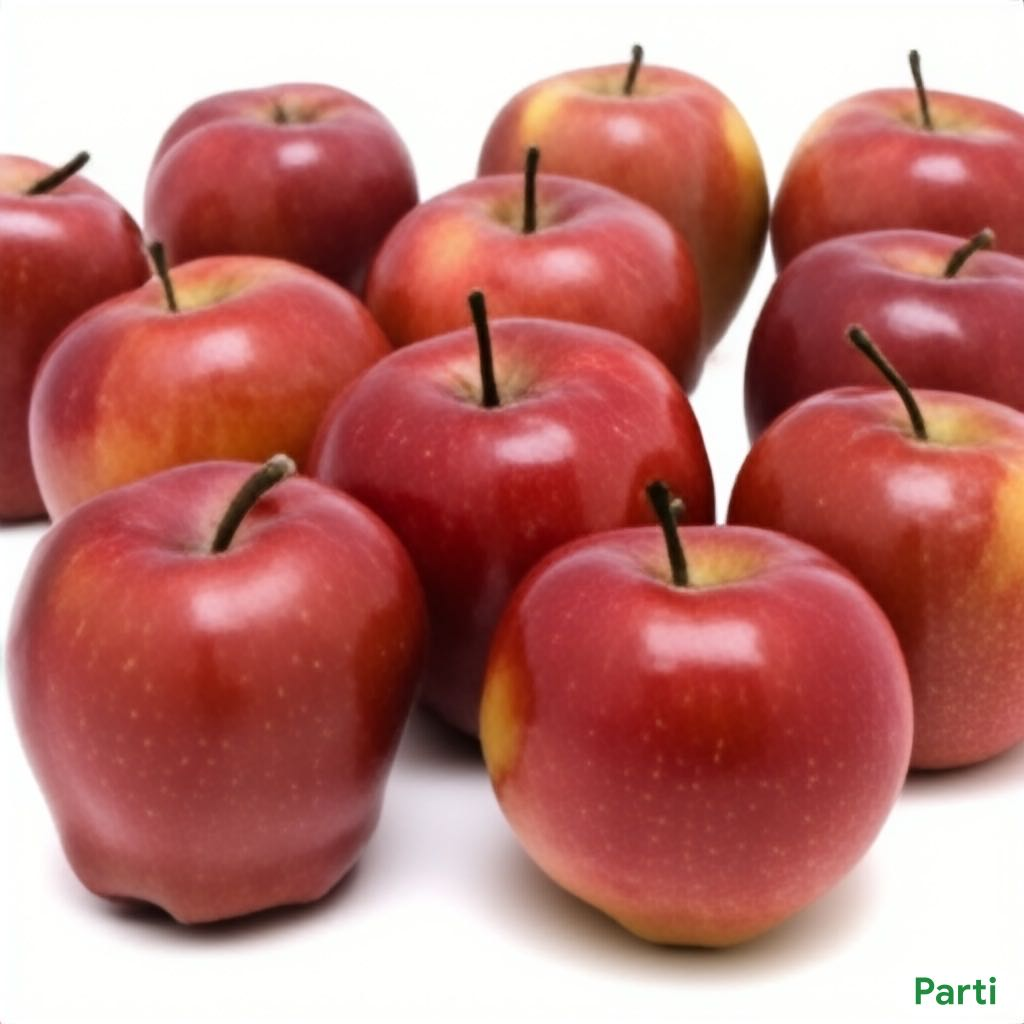
\includegraphics[width=\twobytwocolwidth\textwidth]{figures/limitations/apples_count11.jpg}} &&
\multicolumn{3}{c}{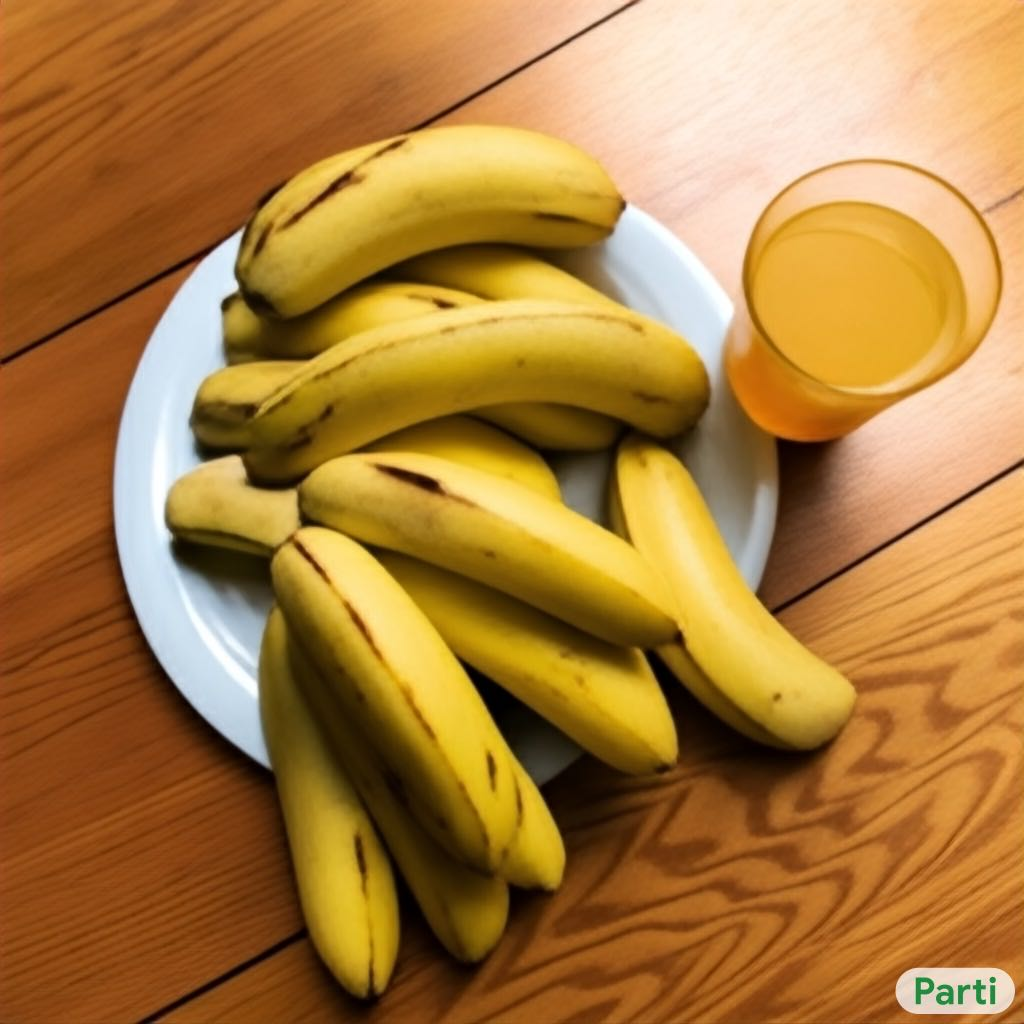
\includegraphics[width=\twobytwocolwidth\textwidth]{figures/limitations/banana_juice_1.jpg}} &
\multicolumn{3}{c}{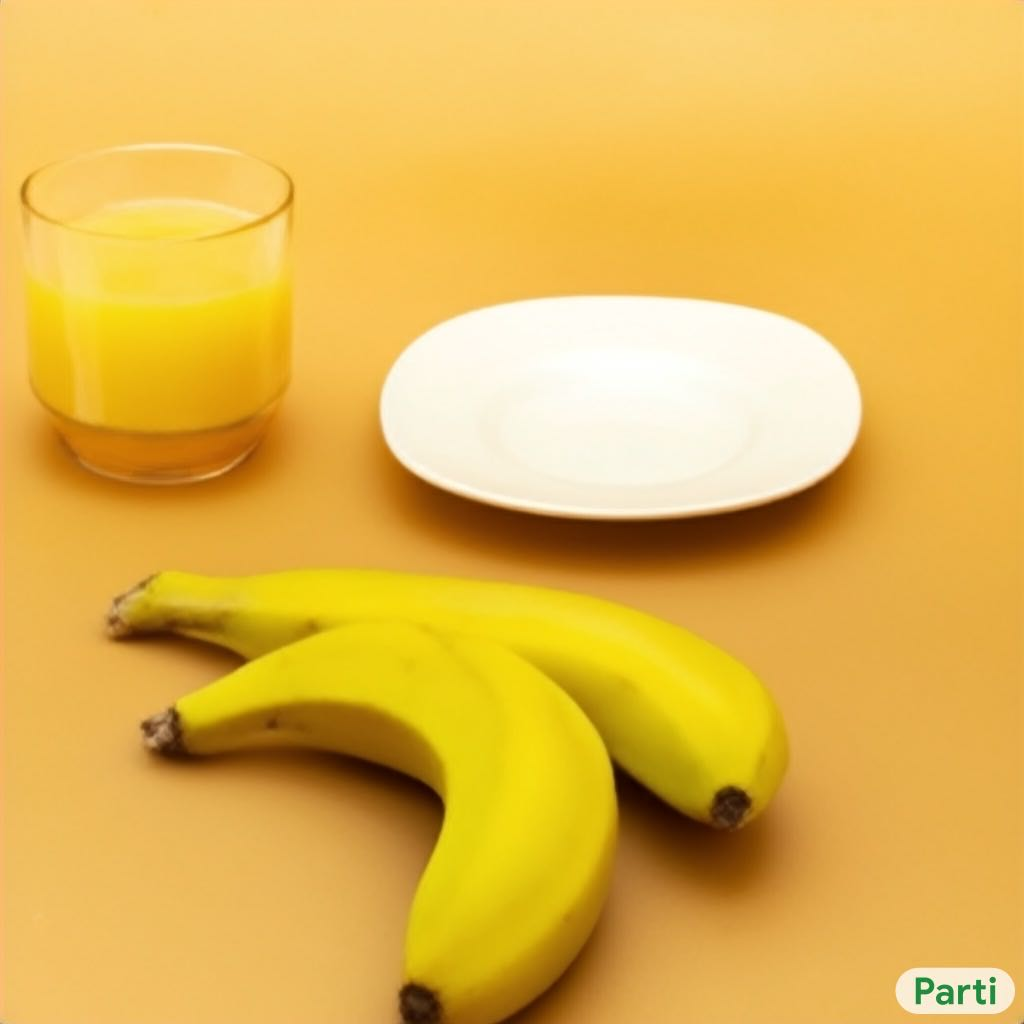
\includegraphics[width=\twobytwocolwidth\textwidth]{figures/limitations/banana_juice_2.jpg}} \\
\multicolumn{6}{C{\thirdcolwidth\textwidth}}{\tiny \textbf{D}. Four images generated in the same batch for the prompt  \textit{A portrait of a statue of Anubis with a crown and wearing a yellow t-shirt that has a space shuttle drawn on it. A white brick wall is in the background.} \textbf{Failures}: color bleeding (a,d); incorrect visual aspect (a,b,d); (unspecified) media blending (c); displaced positioning (b,d); missing details (a,c).} && 
\multicolumn{6}{C{\thirdcolwidth\textwidth}}{\tiny \textbf{E}. (a,b) Two images generated in the same batch for  \textit{a cream colored labradoodle next to a white cat with black-tipped ears}. (c,d) Two images generated in the same batch for \textit{ten red apples}. \textbf{Failures}: hard to disentangle specific features assigned to multiple entities in the same description (a,b); incorrect count of 8 (a) and 11 (b). (Note that some correctly had ten apples.)} && 
\multicolumn{6}{C{\thirdcolwidth\textwidth}}{\tiny \textbf{F}. (a, b) Two images in the same batch for the prompt  \textit{a stack of three red cubes with a blue sphere on the right and two green cones on the left}. (c, d) Two images in the same batch for the prompt \textit{a plate that has no bananas on it. there is a glass without orange juice next to it.} \textbf{Failures}: Incorrect relative positioning of objects (a,b,d). Incorrect coloring-to-attribute association (b). Hallucination (of objects specifically mentioned as absent) (c, d).} \\

\multicolumn{3}{c}{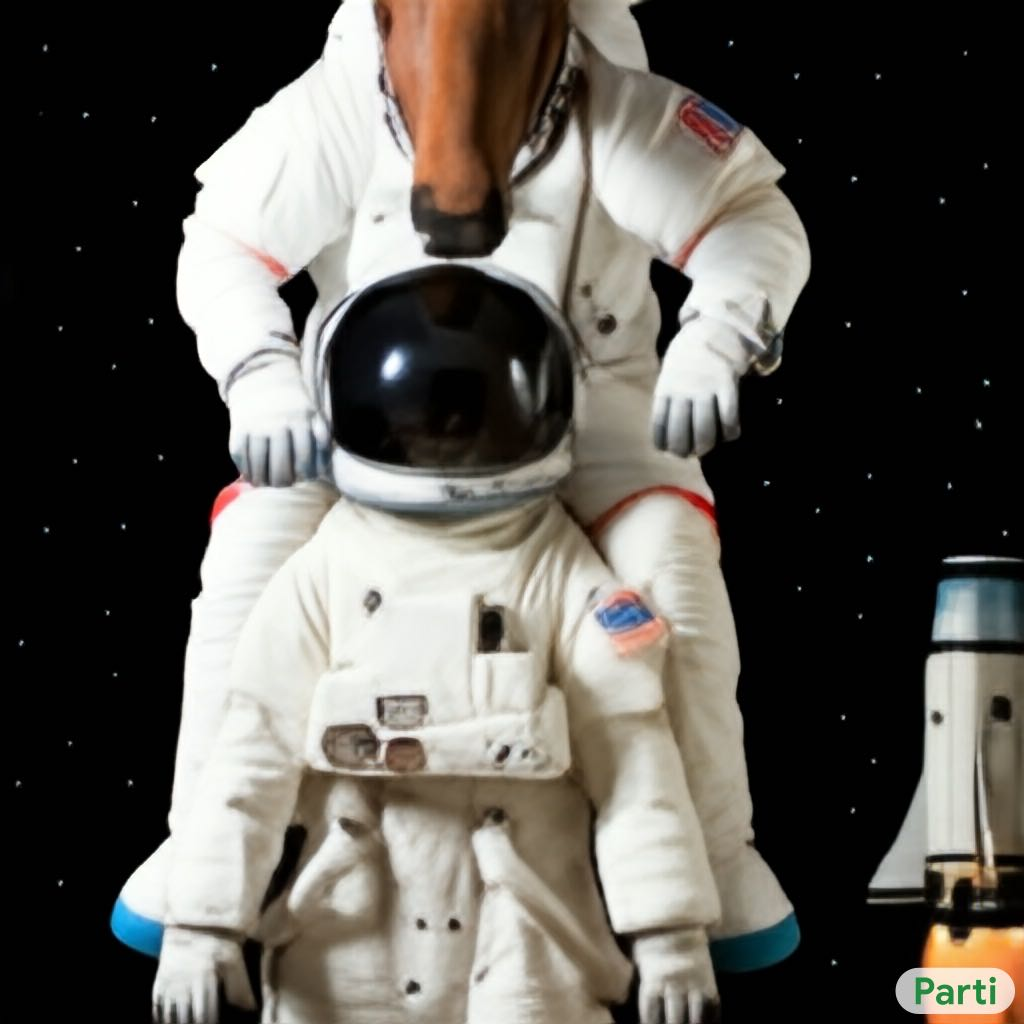
\includegraphics[width=\twobytwocolwidth\textwidth]{figures/limitations/astrohorse1.jpg}} &
\multicolumn{3}{c}{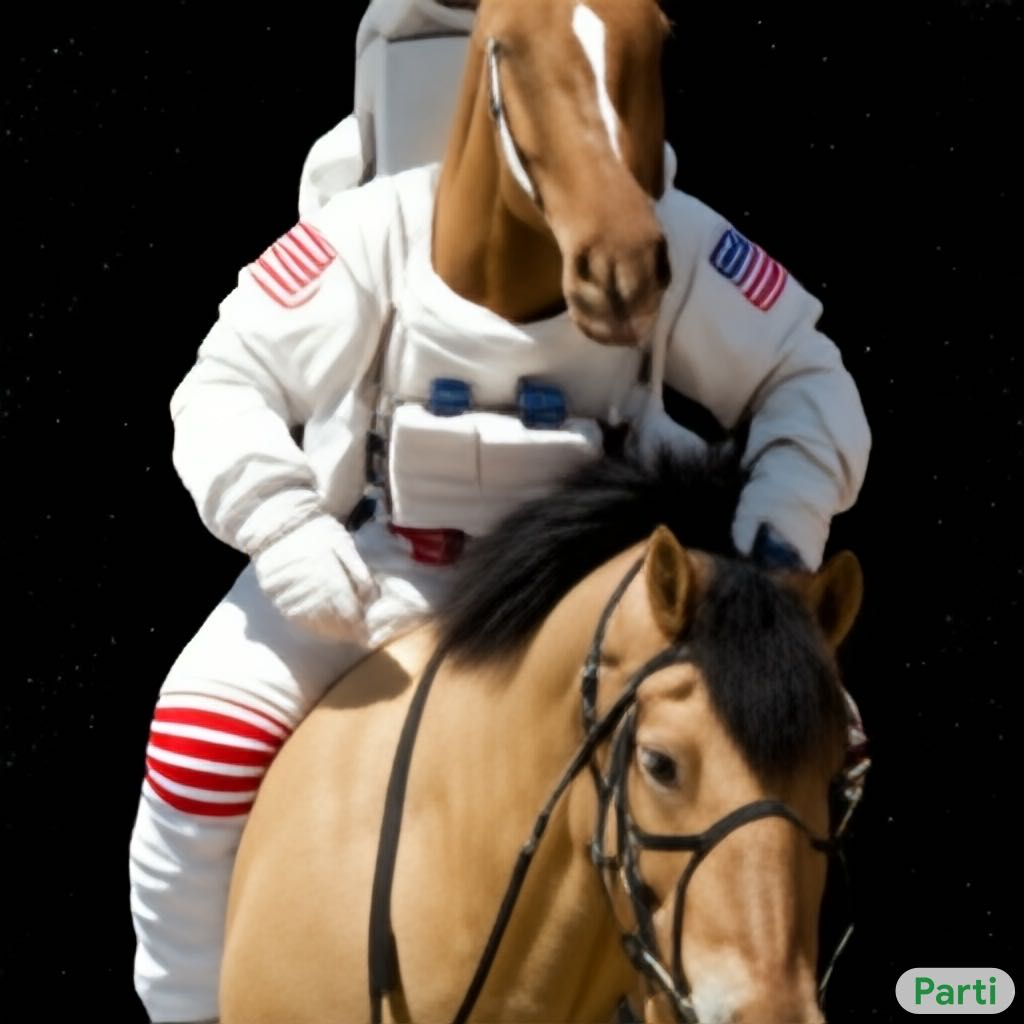
\includegraphics[width=\twobytwocolwidth\textwidth]{figures/limitations/astrohorse2.jpg}} &&
\multicolumn{3}{c}{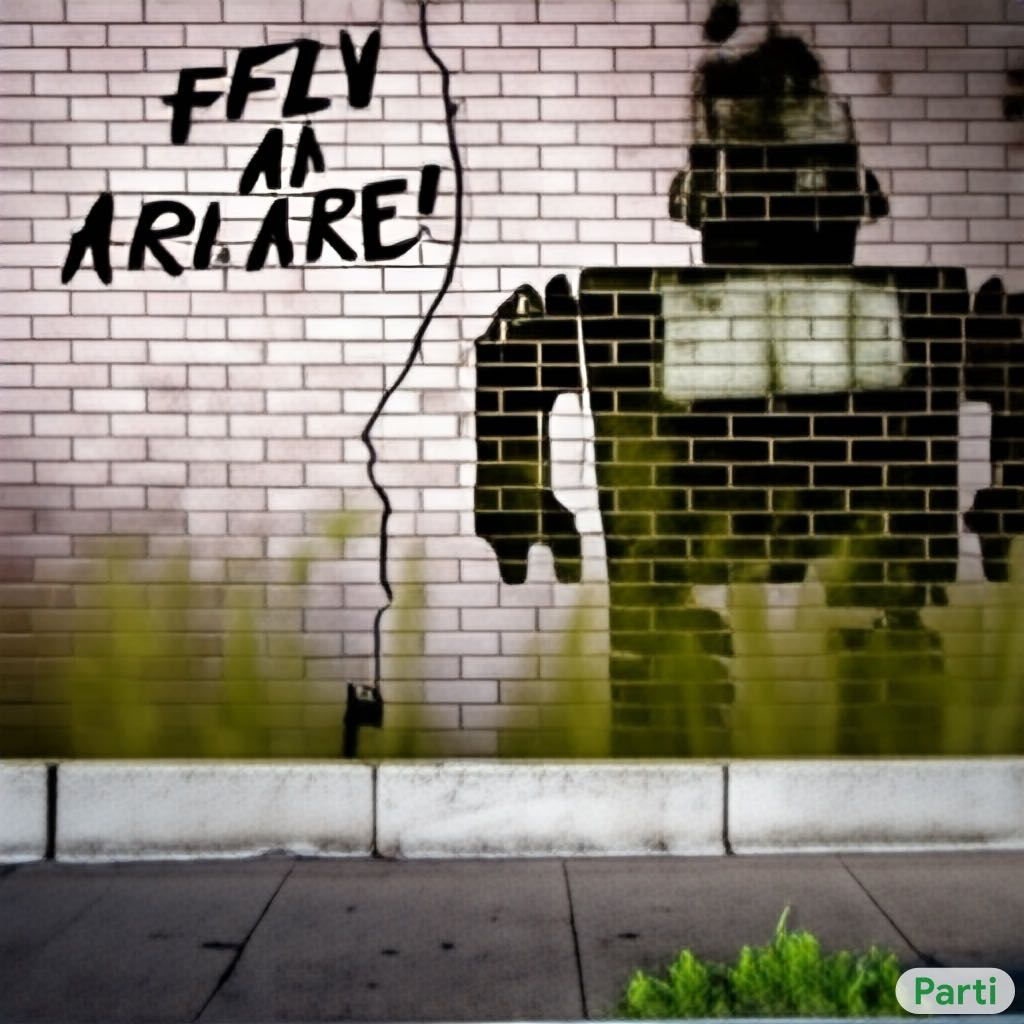
\includegraphics[width=\twobytwocolwidth\textwidth]{figures/limitations/robot_airplane1.jpg}} &
\multicolumn{3}{c}{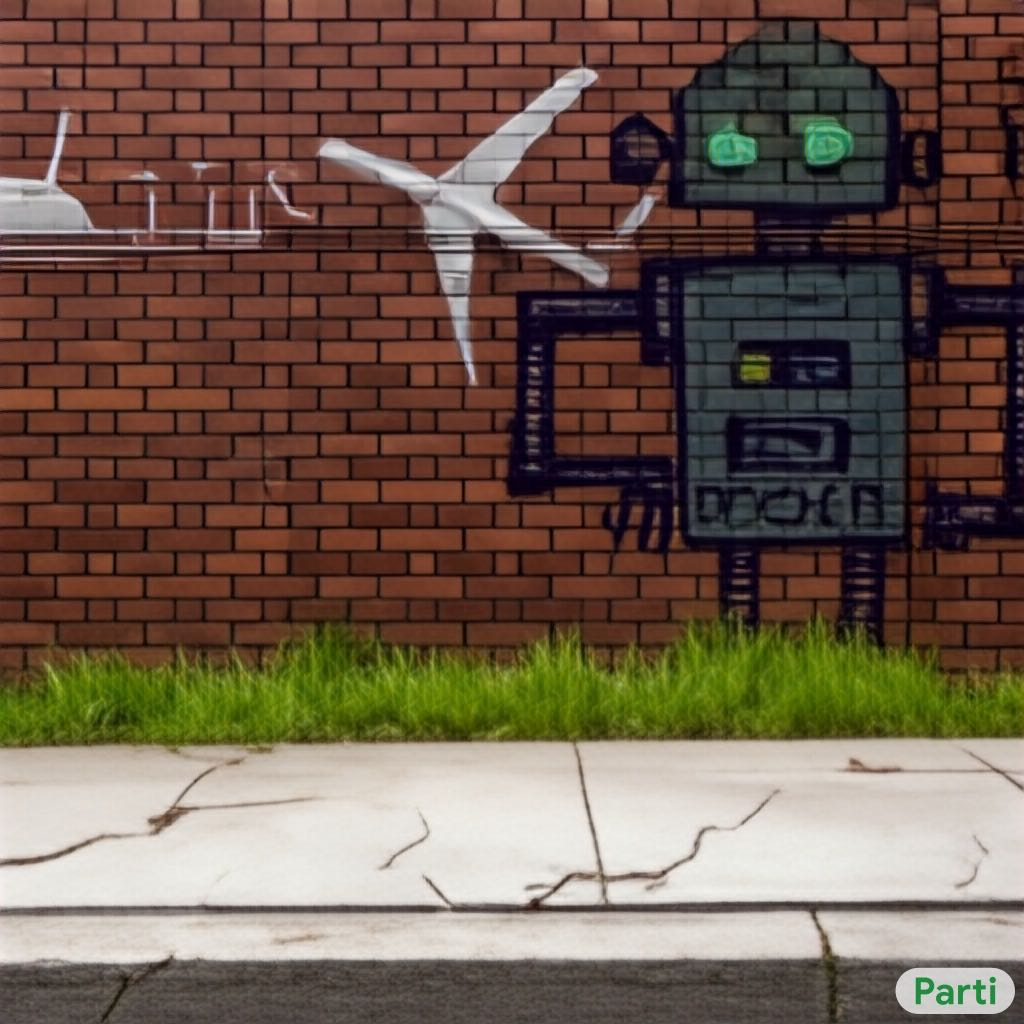
\includegraphics[width=\twobytwocolwidth\textwidth]{figures/limitations/robot_airplane2.jpg}} &&
\multicolumn{3}{c}{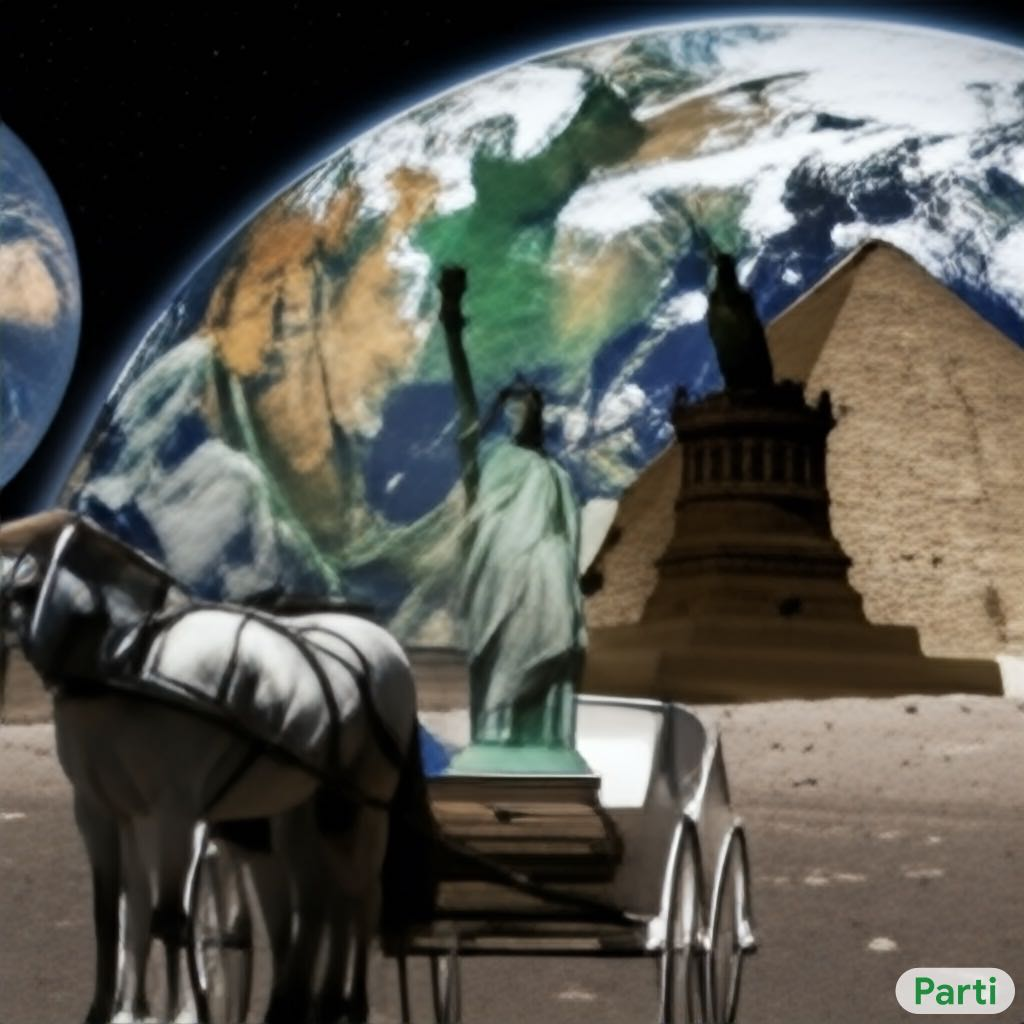
\includegraphics[width=\twobytwocolwidth\textwidth]{figures/limitations/moon_impossible1.jpg}} &
\multicolumn{3}{c}{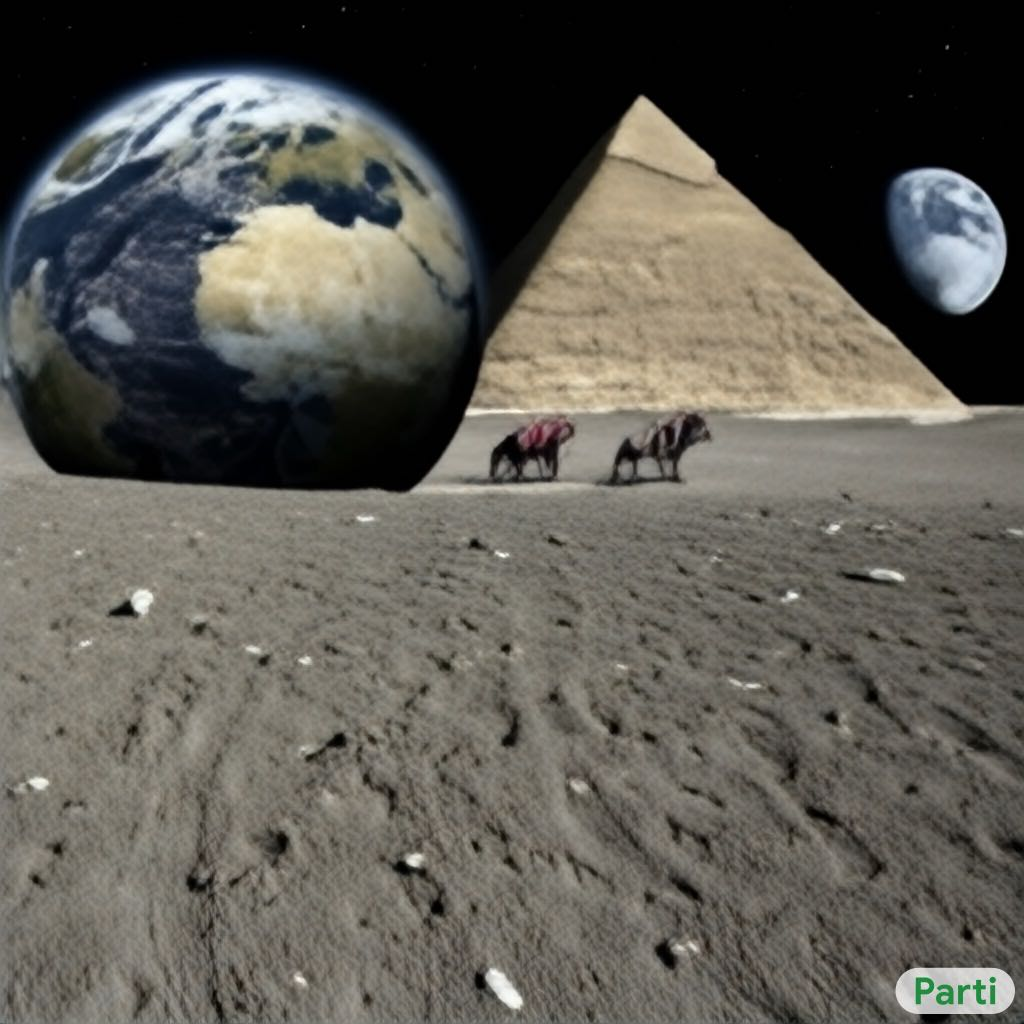
\includegraphics[width=\twobytwocolwidth\textwidth]{figures/limitations/moon_impossible2.jpg}} \\
\multicolumn{3}{c}{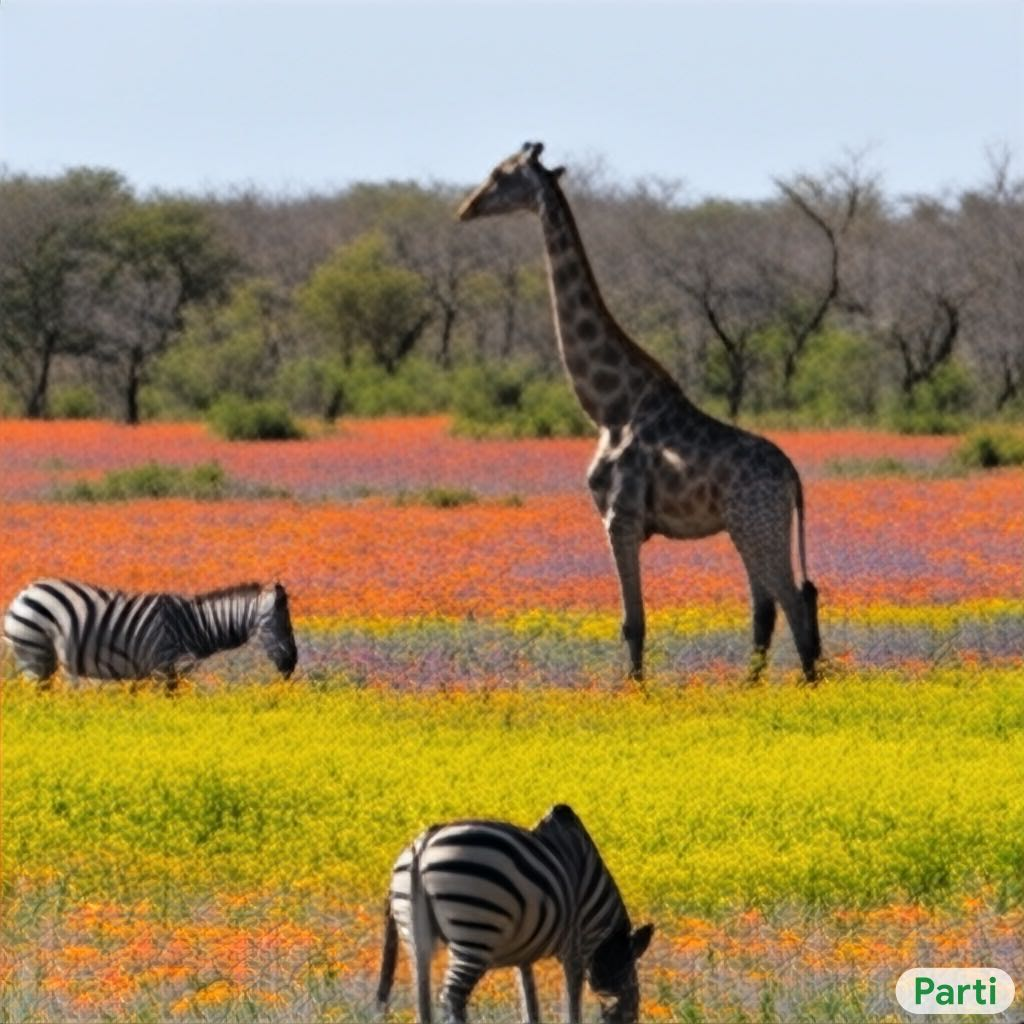
\includegraphics[width=\twobytwocolwidth\textwidth]{figures/limitations/giraffe_zebra3.jpg}} &
\multicolumn{3}{c}{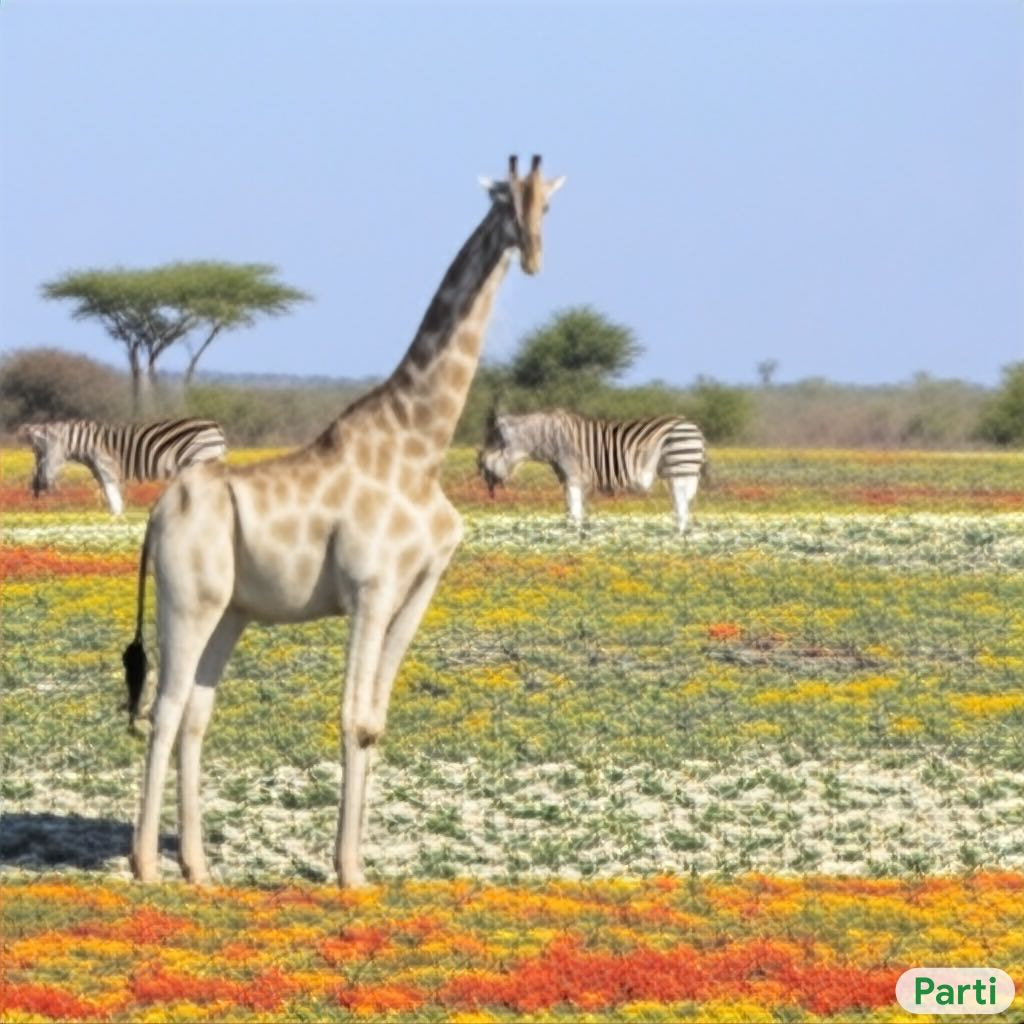
\includegraphics[width=\twobytwocolwidth\textwidth]{figures/limitations/giraffe_zebra4.jpg}} &&
\multicolumn{3}{c}{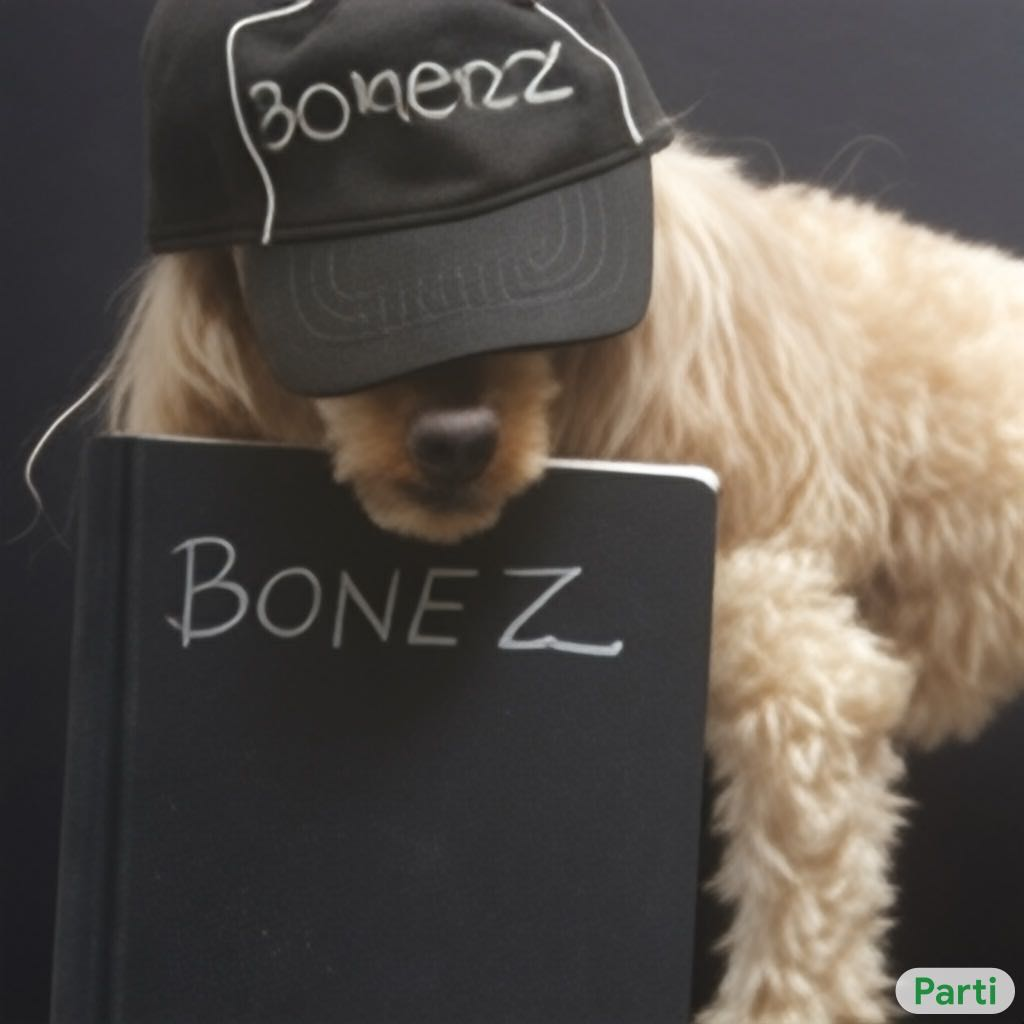
\includegraphics[width=\twobytwocolwidth\textwidth]{figures/limitations/poodle_board3.jpg}} &
\multicolumn{3}{c}{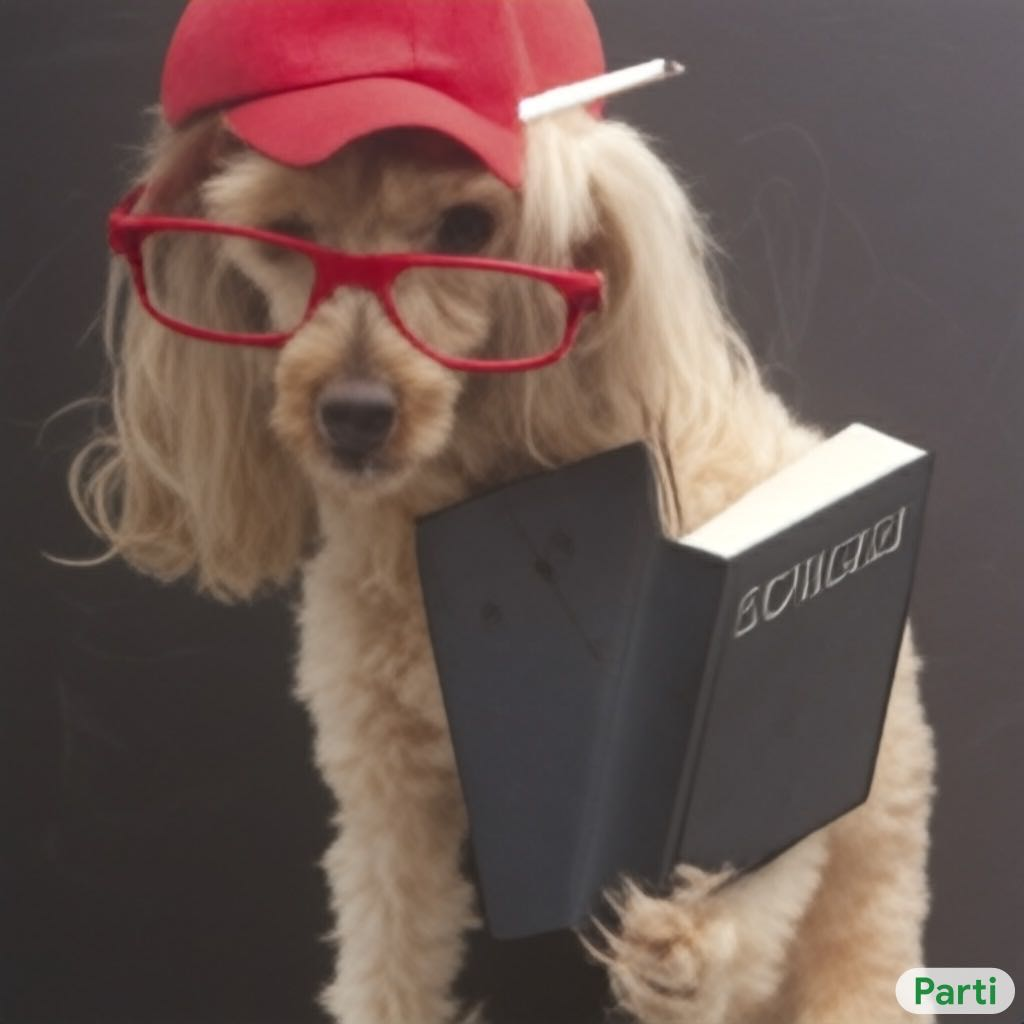
\includegraphics[width=\twobytwocolwidth\textwidth]{figures/limitations/poodle_board4.jpg}} &&
\multicolumn{3}{c}{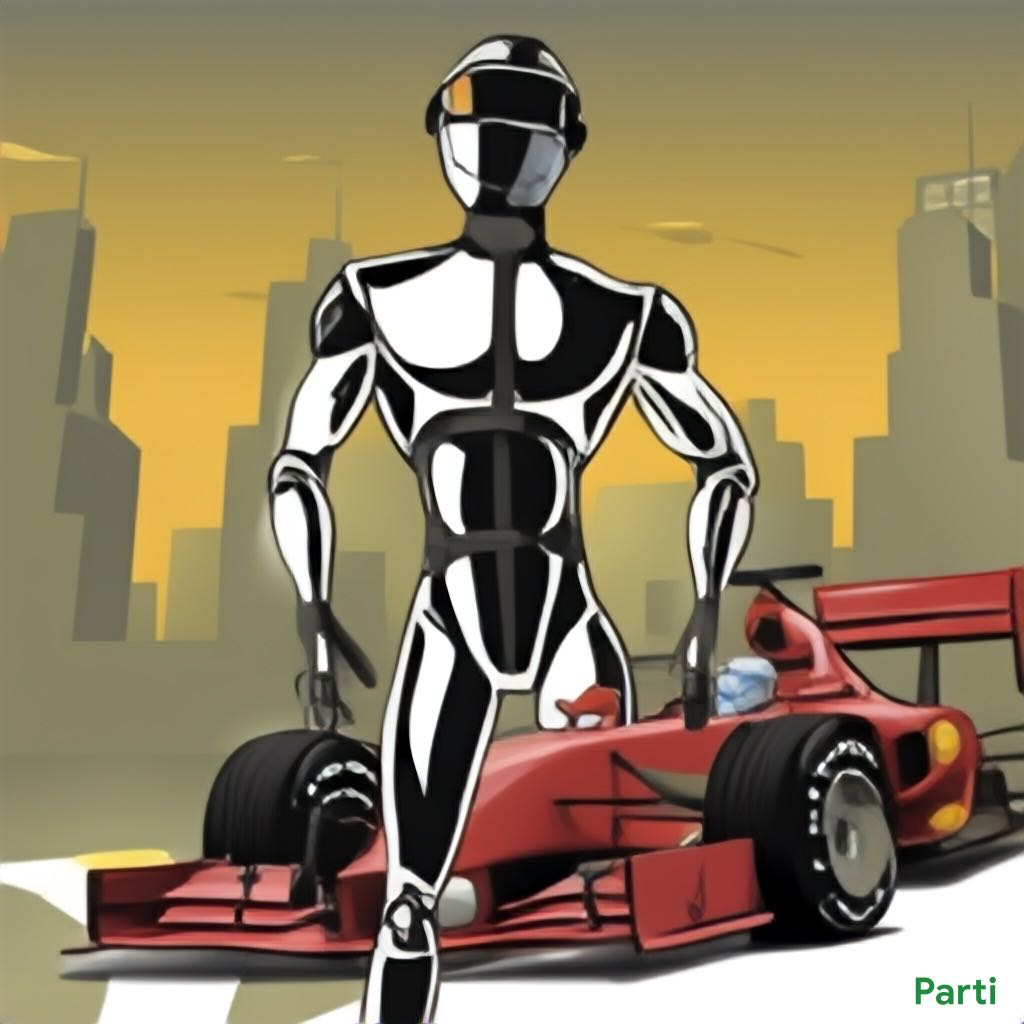
\includegraphics[width=\twobytwocolwidth\textwidth]{figures/limitations/robot_impossible.jpg}} &
\multicolumn{3}{c}{
\includegraphics[width=\twobytwocolwidth\textwidth]{figures/limitations/alien_impossible.jpg}} \\
\multicolumn{6}{C{\thirdcolwidth\textwidth}}{\tiny \textbf{G}. (a,b) Two images in the same batch for \textit{A horse sitting on an astronaut's shoulders. DSLR photo.} (c,d) Two images in the same batch for \textit{Zoomed out view of a giraffe and a zebra in the middle of a field covered with colorful flowers} \textbf{Failures}: hallucination (a); difficulty overriding strong priors (b); entity overriding (another horse instead of an astronaut) (b); entity duplication (zebras) (c,d).} && 
\multicolumn{6}{C{\thirdcolwidth\textwidth}}{\tiny \textbf{H}. (a,b) Two images generated in the same batch for \textit{A robot painted as graffiti on a brick wall. The words "Fly an airplane" are written on the wall. A sidewalk is in front of the wall, and grass is growing out of cracks in the concrete.} (c,d) Two images for \textit{a poodle wearing a baseball cap holding a dictionary in hand and writing bonez on a chalkboard} \textbf{Failures}: Errors/omissions in rendering text (all); use-mention confusion for words (b); incorrect visual aspect (grass)(a); displaced positioning (cracks) (a); hallucination (d).} && 
\multicolumn{6}{C{\thirdcolwidth\textwidth}}{\tiny \textbf{I}. (\textit{See main text for full prompts}) (a,b) Two images generated for a complex prompt of horses pulling a carriage, the statue of liberty, the moon, and the Earth, and images for (c) a robot race car driver and (d) alien graffiti with writing. \textbf{Failures}: Duplication of objects (a,b); relative scaling errors (a,b,c); physically impossible configurations (b,c,d); (unspecified) media blending (d).} \\


\end{tabular}
\end{adjustwidth}
\caption{Images from 20B \bdraw model showing errors and limitations. In the captions, (a), (b), (c), (d) refer to top left, top right, bottom left and bottom right, respectively. Note that many of the example images come from batches that included successful (and typically more highly ranked) images. See Section \ref{secs:limitations} for detailed discussion.}
\label{figs:limitations}
\end{figure}
